\documentclass[12pt]{ociamthesis}  % default square logo 
%\documentclass[12pt,beltcrest]{ociamthesis} % use old belt crest logo
%\documentclass[12pt,shieldcrest]{ociamthesis} % use older shield crest logo

%load any additional packages
\usepackage{amssymb}
\usepackage{multirow}

%input macros (i.e. write your own macros file called mymacros.tex 
%and uncomment the next line)
%\include{mymacros}

\title{\large ANALISIS APLIKASI DOWNLOADER MP4 YOUTUBE  \\[3ex]     %your thesis title,
        \textit{Proyek} I}   %note \\[1ex] is a line break in the title

\author{Irfan Hernandes Panjaitan \\ Kurnia Hayati}             %your name
\college{1.18.4.014 \\ 1.18.4.009 \\[5ex]
\textit{Dalam Pemenuhan Sebagian Persyaratan untuk
Tingkat Sarjana Terapan Teknik Informatika}} %your college

%\renewcommand{\submittedtext}{change the default text here if needed}
\degree{Politeknik Pos Indonesia}     %the degree
\degreedate{Bandung}         %the degree date
\degreedate{2019}  

%end the preamble and start the document
\begin{document}

%this baselineskip gives sufficient line spacing for an examiner to easily
%markup the thesis with comments
\baselineskip=18pt plus1pt

%set the number of sectioning levels that get number and appear in the contents
\setcounter{secnumdepth}{3}
\setcounter{tocdepth}{3}


\maketitle                  % create a title page from the preamble info
\begin{dedication}

”Pendidikan adalah paspor untuk masa,untuk hari esok yang dimiliki oleh orang yang mempersiapkan hari ini. \\
(Malcolm X) \\
Barangsiapa tidak mau merasakan pahitnya belajar, ia akan merasakan hinanya kebodohan sepanjang hidupnya, \\ 
(imam Syafi'i rahimahullah) \\

\end{dedication}        % include a dedication.tex file
\begin{acknowledgements}
Assalamualaikum warahmatullahi wabarakatuh. Segala puji bagi Allah SWT yang telah memberikan kemudahan sehingga dapat menyelesaikan laporan Analisis Proyek 1 ini, tanpa pertolongan-Nya mungkin penulis tidak akan sanggup menyelesaikannya dengan baik. Shalawat dan salam semoga terlimpah curahkan kepada Nabi Muhammad SAW beserta sahabat dan keluarga Beliau.

Laporan ini disusun untuk memenuhi kelulusan matakuliah Proyek 1 pada Program Studi DIV Teknik Informatika. Proses Proyek 1 ini juga tidak terlepas dari bantuan pihak Pembimbing. Oleh karena itu, pada kata pengantar ini penulis menyampaikan teriamakasih kepada :
\begin{enumerate}

\item Rolly Maulana Awangga, S.T., M.T.I. selaku Pembimbing Internal dan Penguji Utama dalam penyusunan laporan Proyek I ini;
\item Nisa Hanum Harani, S.KOM.,M.T selaku Penguji Pendamping dalam sidang Proyek I ini;
\item Nyi Raden Nuraini Siti Fathonah, M.Hum selaku Koordinator Proyek I Tahun Akademik 2018/2019;
\item M. Yusril Helmi Setyawan, S.Kom., M.Kom. selaku Ketua Program Studi DIV Teknik Informatika Tahun Akademik 2018/2019;
\item  Dr. Ir. Agus Purnomo, M.T. selaku Direktur Politeknik Pos Indonesia Tahun Akademik 2018/2019.
\end{enumerate}

Penulis telah membuat laporan ini dengan sebaik-baiknya, diharapkan memberikan kritik dan saran dari semua pihak yang bersifat membangun, terimakasih.

\begin{raggedleft}

Bandung, 20 September 2019

Penulis

\end{raggedleft}

\end{acknowledgements}   % include an acknowledgements.tex file
\begin{abstract}
\textit Android adalah sistem operasi untuk telepon seluler yang berbasis linux. Android menyediakan \textit{Platform} terbuka bagi pengembangan untuk menciptakan suatu aplikasi untuk digunakan oleh berbagai macam perangkat  \textit{Mobile}. Android merupakan kode komputer yang bisa di distribusikan secara terbuka \textit{(Open Source)}, sehingga pengembangan bisa membuat ribuan aplikasi baik yang gratis maupun berbayar. Aplikasi Downloader MP4 Youtube adalah salah satu aplikasi downloader video yang disediakan untuk mempermudah user dalam mengunduh video dan musik dengan mudah serta efisien. Aplikasi ini juga disediakan secara gratis. Analisi ini bertujuan mengetahui sitem kerja dari aplikasi Downloader MP4 Youtube dan Attribut yang ada dalam proses penggunaan dalam aplikasi.


\textbf{Kata kunci :} Android, Platform, Open Source, Aplikasi, Mobile, Attribut. 
\end{abstract}          % include the abstract
\begin{abstract}
\textit{Android is an operating system for Linux-based cellular phones. Android provides an open \textit platform for development to create an application for use by a variety of \textit Mobile devices. Android is a computer code that can be publicly distributed \textit {(Open Source)} so that development can create thousands of applications both free and paid. MP4 Download Application Youtube is a video download application provided to facilitate users in downloading videos and music easily and efficiently. This application is also provided free of charge. This analysis aims to find out the work system of the MP4 Youtube Download application and the attributes that exist in the process of using the application.}



\textbf{Keywords:} \textit {Android, Platform, Open Source, Application, Mobile, Attributes.}
\end{abstract}

\begin{romanpages}          % start roman page numbering
\tableofcontents            % generate and include a table of contents
\listoffigures
\listoftables           % generate and include a list of figures
\end{romanpages}            % end roman page numbering

%now include the files of latex for each of the chapters etc
\chapter{PENDAHULUAN}

\section{Latar Belakang}
Perkembangan Aplikasi pada saat ini telah mengalami peningkatan yang sanggat drastis \cite{neyfa2016perancangan}. Hal tersebut dapat didukung dengan adanya kemudahan aplikasi saat ini yang bermacam-macam salah satunya yaitu Downloader MP4 Youtube (savefrom.net). Aplikasi Downloader MP4 Youtube Merupakan aplikasi download video yang popular digunakan oleh pengguna komputer atau laptop. Selain pengguan komputer dan laptop, aplikasi Downloader Mp4 juga disediakan di android. Aplikasi Downloader Mp4 tidak hanya tersedia dalam bentuk aplikasi tetapi juga tersedia dalam bentuk web \cite{neyfa2016perancangan} . Aplikasi Downloader Mp4 ini digunakan sebagai media mendownload video tanpa adanya batasan ukuran. Selain itu aplikasi ini menyediakan berbagai macam kualitas  seperti Mp4 atau WEBN dan banyak lagi. Dengan adanya kecanggihan tersebut aplikasi ini memudahkan user ketika menggunakannya dalam sehari-hari serta aplikasi ini sangat mudah dalam penggunaannya. 


\section{Identifikasi Masalah}
Berdasarkan latar belakang masalah yang ada, maka dapat diidentifikasi menjadi beberapa masalah sebagai berikut:
\begin{enumerate}
\item Bagaimana penerapan fungsi serta algoritma dan pemograman dalam metode download pada Aplikasi ?
\end{enumerate}

\section{Tujuan}
Berdasarkan latar belakang dan identifikasi masalah yang ada, maka akan memberikan tujuan dan manfaat sebagai berikut:
\begin{enumerate}
\item Mengetahui bagaimana sistem yang berjalan dari awal pencarian video hingga mendownload video pada  aplikasi Downloader Mp4 Youtube ( savefrom.net ) dengan bantuan selenium.
\item Mengetahui bagaimana menjalankan sebuah program secara otomatis pada aplikasi Download Mp4 Youtube (savefrom.net) dengan bantuan selenium.
\end{enumerate}

\section{Ruang Lingkup}
Dari data – data yang didapatkan dari proses identifikasi masalah ini maka ruang lingkup dari penelitian ini adalah sebagai berikut:
\begin{enumerate}
\item Sistem cara pengunduhan video dari aplikasi Downloader Mp4 Youtube.
\end{enumerate}

\section{Sistematika Penulisan}
Materi-materi yang tertera pada Laporan Proyek 1 ini dikelompokkan menjadi beberapa sub bab dengan sistematika penyampaian sebagai berikut :
\begin{enumerate}
    \item BAB 1 PENDAHULUAN
    \par
    Pada bab ini berisi latar belakang,identifikasi masalah,tujuan,ruang lingkup dan sistematika penulisan.
    
    \item BAB 2 LANDASAN TEORI
    \par
    Pada bab ini berisi tentang teori yang berupa pengertian atau definisi sistem penggunakan aplikasi Downloader Mp4 Youtube(savefrom.net).
    
    \item  BAB 3 ANALISIS DAN PERANCANGAN
    \par
    Pada bab ini akan dijelaskan function algoritma yang digunakan pada program / sistem aplikasi dan akan dijelaskan bagaimana alur kerja program aplikasi yang akan digambarkan dalam bentuk flowmap sehingga pembaca akan lebih mudah mengerti analisis ini.
    
    \item BAB 4 IMPLEMENTASI
    \par
    Bab ini menjelaskan tentang implementasi yang terdiri dari alat pendukung serta aplikasi pendukung ,lingkungan implementasi, tampilan antar muka, dan petunjuk pemakaian. Bab ini juga membahas tentang pembahasan hasil pengujian.
    
    \item BAB 5 KESIMPULAN DAN SARAN
    \par
    Bab ini berisi kesimpulan dan saran yang berkaitan dengan analisis yang telah dituliskan pada bab sebelumnya sehingga pembaca lebih mudah mengerti hasil dari analisis yang telah dilakukan dan penulis juga dapat memberikan saran di bab ini.

\end{enumerate} 
\chapter{Tinjauan Pustaka}

\par
Dalam suatu analisis diperlukan dukungan hasil-hasil analisis yang telah ada sebelumnya yang berkiatan dengan penetian tersebut.

Menurut Dwi Prastowo Darminto {(2002;52)} Analisi adalah Penguraian suatu pokok atas berbagai bagiannya dan menelaah bagian itu sendiri serta hubungan antar bagian untuk memperoleh pengertian yang tepat dan pemahaman arti keseluruhan.

Menurut Komaruddin {(2001:53)} Pengertian analisis adalah kegiatan berpikir untuk menguraikan suatu keseluruhan menjadi komponen sehinga dapat mengenal tanda-tanda komponen, hubungannya satu sama lain dan fungsi masing-masing dalam satu keseluruhan yang terpadu.

Dengan demikian, bisa disimpulkan bahwa pengertian analisis yaitu suatu prosedur tahapan pekerjaan yang akan didokumentasikan dengan tahapan pembuatan laporan agar mudah dalam pemahaman.

\section{Selenium}
Selenium adalah perangkat lunak yang berfungsi untuk mendukung
pengembangan otomatisasi uji berbasis web aplikasi. Selenium menyediakan pengujian khusus terhadap domain bahasa,untuk melakukan tes menulis pada beberapa bahasa pemrograman yan populer, termasuk C\#, Groovy, Java, Pearl,PHP, Python, Ruby, dan juga Scala \cite{razak2011agile}. Pengujian dapat berjalan melalui browser web apa saja dan dapat dilakukan melalui Sistem Operasi di Windows, Linux, dan Platform OS X. Selenium Python Bindings menyediakan API yang sederhana untuk menulis uji fungsional menggunakan Selenium WebDriver, dan juga dapat mengakses semua fungsi Selenium WebDriver secara intuitif. Selenium Python Bindings menyediakan API yang cukup nyaman untu melakukan suatu akses Selenium WebDrivers seperti di Firefox, Internet Explorer, Chrome, dll
Ada beberapa alat Selenium untuk otomasi perangkat lunak diantaranya,Selenium IDE, Selenium RC, dan Selenium WebDriver.

\subsection{Selenium IDE}
Selenium IDE adalah lingkungan pengembangan yang terintegrasi untuk membangun suatu skrip yang akan diujikan. Ini adalah suatu plug-in Firefox yang memungkinkan merekam edit dan juga men-debug suatu kasus uji di selenium\cite{razak2011agile}. Ini mencatat semua tindakan yang dilakukan oleh pengguna yang skrip pengujian. Fitur yang terdapat pada Selenium IDE yaitu: Kemudahan untuk recorcd dan playback, Seleksi field yang pintar menggunakan id, nama, class, XPath dan lainnya sesuai kebutuhan, Auto complete untuk semua perintah selenium yang umum, wakl through test (step by step), debug dan pengaturan breakpoint, menyimpan script test sebagai HTML, Phyton, Ruby, dan format lain, Mensupport file Selenium user-extensions.js, OPsi untuk secara otomatis mengecek judul setiap halaman, kemudahan melalui plugins.

\subsection{Remote Control Selenium}{(RC)}
Remote Control Selenium (RC) adalah selenium utama yang digunakan untuk memproyeksikan waktu yang lama. Selenium RC lebih lambat daripada selenium webdriver karena menggunakan program java script yang disebut sebagai suatu inti dari selenium \cite{maruyama1994wireless}. Selenium RC harus memulai server sebelum menjalankan suatu skrip pengujian, dan itu tidak mendukung untuk aplikasi Ajax. Cara menghindari keterbatasan Selenium RC, yaitu dengan selenium WebDriver. Selenium RC terdiri dari dua bagian yaitu:
\begin{enumerate}
    \item Server yang secara otomatis menjalankan dan menghentikan web browser, dan bertindak sebagai HTTP proxy untuk setiap web request. Server menggunakan java.
    \item Librari Client untuk Bahasa pemograman Java, Python, PHP, Perl, Ruby, dan C\#.
\end{enumerate}

\subsection{Selenium WebDriver}
Secara langsung berkomunikasi dengan browser, jadi selenium WebDriver menyebabkan lebih cepat daripada Selenium RC. Selenium WebDriver mendukung beberapa browser web dan juga mendukung untuk aplikasi Ajax \cite{razak2011agile}. Tujuan utama dari Selenium WebDriver untuk meningkatkan dukungan modern masalah pengujian aplikasi di berbagai web, dan juga mendukung berbagai bahasa untuk menulis suatu skrip pengujian. Terlepas dari semua keunggulan Selenium WebDriver, ia memiliki keterbatasan pada saat menguji suatu aplikasi web, karena tidak memiliki fungsionalitas untuk menghasilkan tangkapan layar dalam kasus uji kegagalan. Selenium WebDriver tidak memiliki kapabilitas bawwan untuk menghasilkan hasil dari tes, dikarenakan tergantung pada pihak alat ketiga untuk menghasilkan laporan pengujian. Keterbatasan ini dapat dihindari dengan menggunakan kerangka TestNG

\subsection{TestNG}
TestNG adalah kerangka kerja pengujian yang dirancang untuk mengatasi keterbatasan kerja dari pengujian Jumlah unit. TestNG mencakup semua kategori tes sebagai unit, fungsional, pengujian integrasi. TestNG menghasilkan laporan pengujian dan menjalankan beberapa tes case secara paralel. Laporan TestNG sangat membosankan untuk diahami, sehingga memerlukan beberapa modifikasi.

\subsection{Selenium Grid}
Server yang memungkinkan pengujian untuk menggunakan instace browser web yang sedang berjalan di mesin jarak jauh. Dengan selenium grid, satu server bertindak sebagai hub\cite{razak2011agile}. Tes hubungi hub untuk mendapatkan akses ke instance browser karena hub memiliki daftar server yang menyediakan akses ke insntance browser (node WebDriver), dan memungkinkan pengujian menggunakan instance ini. Selenium Grid memiliki kemampuan untuk menjalankan tes pada instance browser jarak jauh yang berguna untuk menyebarkan beban pengujian di beberapa mesin, dan untuk menjalankan tes di browser yang berjalan pada platform atau sistem operasi yang berbeda. Yang terakhir ini sangat berguna dalam kasus di mana tidak semua browser yang akan digunakan untuk pengujian dapat berjalan pada platform yang sama.

\subsection{Selenium Core}
Bagian yang melakukan playback pada web browser yang sebenarnya.

\subsection{Analisis Sistem}
Analisis sistem adalah penelitian terhadap sebuah sistem dengan tujuan mengevaluasi berbagai macam masalah maupun hambatan yang muncul pada sistem aplikasi yang nantinya dapat dilakukan perbaikan atau pengembangan \cite{aini2007sistem}. Analisis penting dalam segala aspek dan sangat dibutuhkan untuk melakukan sebuah penelitian maupun pengembangan. Kemampuan dalam menganalisa suatu sistem juga diperlukan saat mempelajari bagaimana proses terciptanya aplikasi dan cara kerja sebuah aplikasi.

\section{Cara Install Selenium}
\begin{enumerate}
    \item Buka cmd, kemudian ketik python dan kemudian enter
    \item Langkah selanjutnya, ketik pip install selenium.
    \item Selanjutnya ketik list, untuk mengecek apakah selenium sudah terinstall di laptop anda

\end{enumerate}

\section{Anaconda}
Anaconda adalah perusahaan pengembang dan juga pengembang perangkat lunak pendukung sumber terbukayang berbasis di Austin, Texas, AS. Berkomitmen untuk open source, dan juga menciptakan distribusi dari Anaconda Python dan berkontribusi pada banyak alat analisis data berbasis sumber terbuka lainnya.

\subsection{Cara Install Anaconda}
Sebelum menginstall Anaconda Python hal pertama yang harus diperhatikan yaitu versi dari Sistem Operasi yang digunakan, misalnya Windows versi 32bit atau 64bit, jadi anda harus menginstall Anaconda Pyton sesuai dengan Sistem Operasi di windows anda, karena jika versi windows dapat menyebabkan error.
\begin{enumerate}
    \item Download Anaconda Python https://www.anaconda.com/distribution/
    \item Jika sudah didownload, buka installer Anaconda
    \begin{figure}[!htbp]
        \centering
        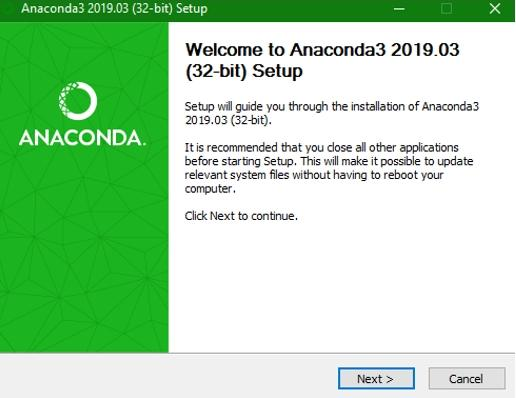
\includegraphics[scale=0.6]{figure/Anaconda/1.jpeg}
        \label{gambar 1}
    \end{figure}
    \vspace{2cm}
    \item Kemudian Pilih lokasi menyimpanan aplikasi
    \begin{figure}[!htbp]
        \centering
        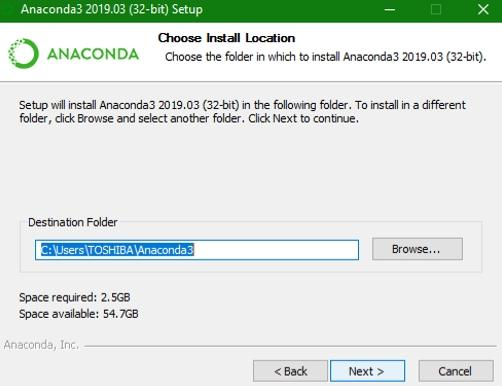
\includegraphics[scale=0.6]{figure/Anaconda/3.jpeg}
        \label{gambar 1}
    \end{figure}
    \item Lalu pilih Just Me(recommended) agar sesuai dengan computer yang ada miliki.
    \begin{figure}[!htbp]
        \centering
        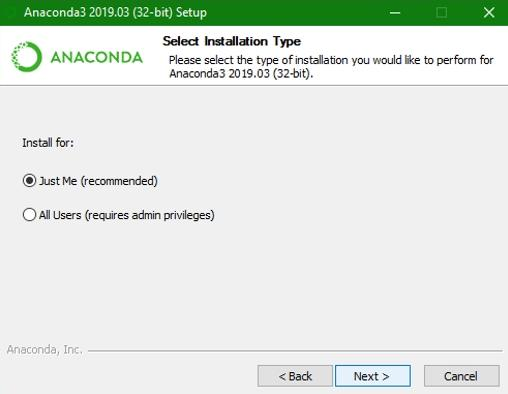
\includegraphics[scale=0.6]{figure/Anaconda/4.jpeg}
        \label{gambar 1}
    \end{figure}
           \vspace{2cm}
    \item Kemudian ceklis Add Anaconda to my PATH
    \item Lalu anda centang Add Anaconda to my Path environment variable, agar saat mengisntall selenium langsung ke path anaconda tidak ke aplikasi yang lain.
    \item Jika sudah klik install, tunggu sampai selesai proses installasi selesai.
    \begin{figure}[!htbp]
        \centering
        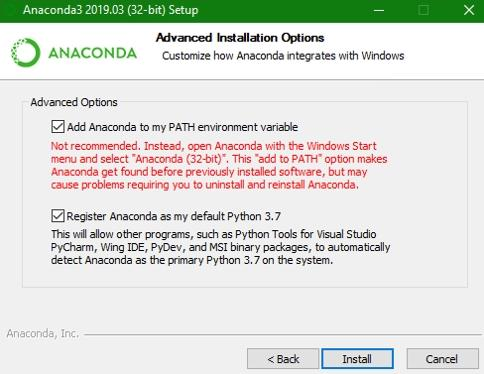
\includegraphics[scale=0.6]{figure/Anaconda/5.jpeg}
        \label{gambar 1}
    \end{figure}
    \item Klik Next  
    \begin{figure}[!htbp]
        \centering
        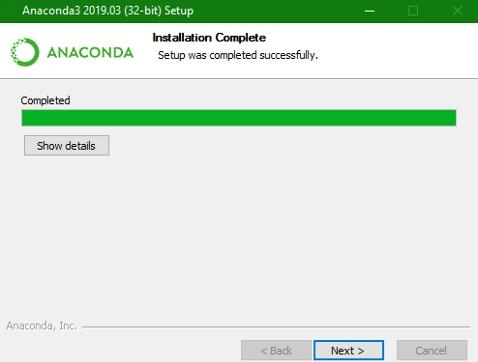
\includegraphics[scale=0.6]{figure/Anaconda/6.jpeg}
        \label{gambar 1}
    \end{figure}
    \vspace{2cm}
    \item Klik Next
    \begin{figure}[!htbp]
        \centering
        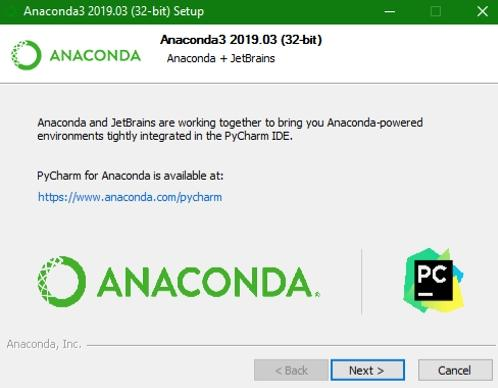
\includegraphics[scale=0.6]{figure/Anaconda/7.jpeg}
        \label{gambar 1}
    \end{figure}
    \item klik Next
    \item Jika sudah selesai Klik Finish
    \begin{figure}[!htbp]
        \centering
        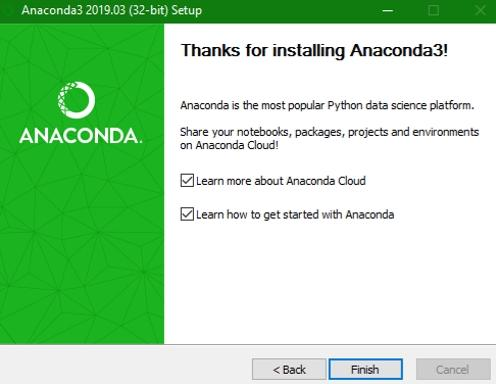
\includegraphics[scale=0.6]{figure/Anaconda/8.jpeg}
        \label{gambar 1}
    \end{figure}
\end{enumerate}
    \vspace{1cm}
\subsubsection{Flowchart}
Pengertian flowchart adalah bagan alir yang menggambarkan prosedur pada suatu sistem dengan simbul-simbol yang memiliki maknanya masing-masing \cite{solikin2018implementasi}. Fungsi dari flowchart yaitu untuk merancang proyek baru, menggambarkan proses bisnis, menggambarkan alur kerja dan menampilkan sebuah algoritma. Berberapa simbol yang ada pada flowchart yakni simbol arus, simbol proses dan simbol input/output. Pada gambar \ref{gambar 1} berikut contoh simbol simbol Flowchart.

\begin{figure}[!htbp]
    \centering
    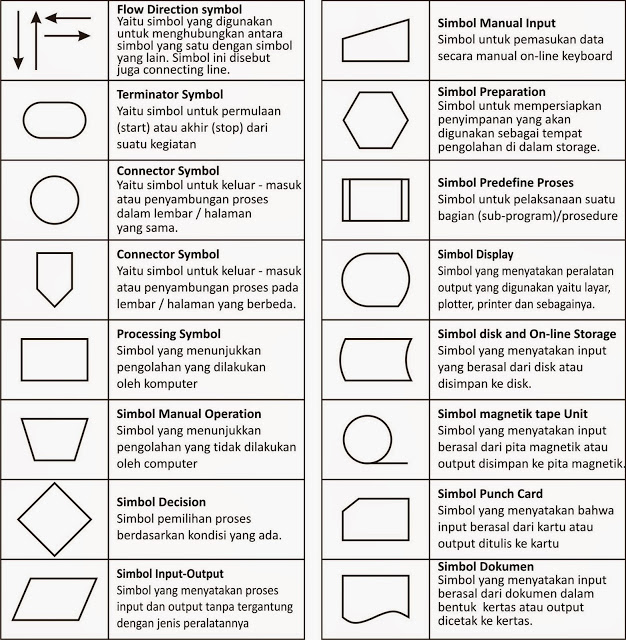
\includegraphics[scale=0.6]{figure/flowchart.jpg}
    \caption{\textit{Simbol Flowchart}}
    \label{gambar 1}
\end{figure}
\vspace{1cm}
\subsubsection{Flowmap}
Flowmap adalah penggambaran secara grafik sebuah prosedur yang ada pada suatu program \cite{rahayu2011perancangan}. Flowmap membantu analisis karena flowmap menggambarkan alur prosedur dan juga algoritma secara grafik. Pada gambar \ref{gambar 2} berikut contoh simbol simbol flowmap.

\begin{figure}[!htbp]
    \centering
    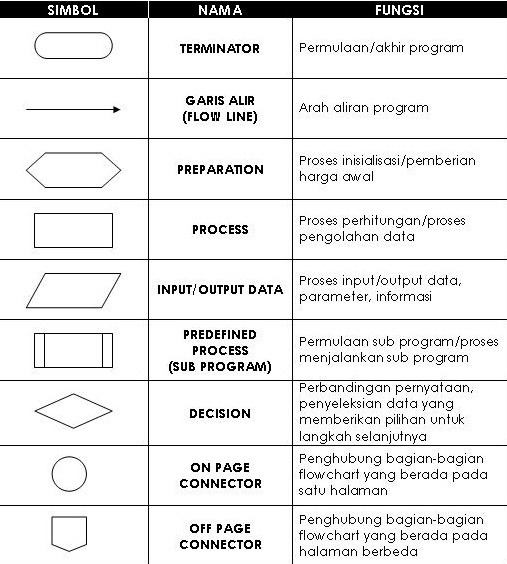
\includegraphics[scale=0.8]{figure/flowmapp.JPG}
    \caption{\textit{Simbol Flowmap}}
    \label{gambar 2}
\end{figure}
\vspace{4cm}
\subsection{Perancangan Sistem}
\subsubsection{Data Flow Diagram (DFD)}
Data Flow Diagram (DFD) adalah bentuk model hasil analisis sebuah kebutuhan dari perangkat lunak \cite{rivai2013pembangunan}. DFD bisa dikatakan sebagai gambaran rancangan sistem dari sebuah program yang berorientasi ke alur data dengan tujuan agar gambaran tersebut mudah dikomunikasikan oleh pembuat sistem atau pembuat program ke pengguna program tersebut.Pada gambar \ref{gambar 3} berikut contoh simbol simbol Dfd.

\begin{figure}[!htbp]
    \centering
    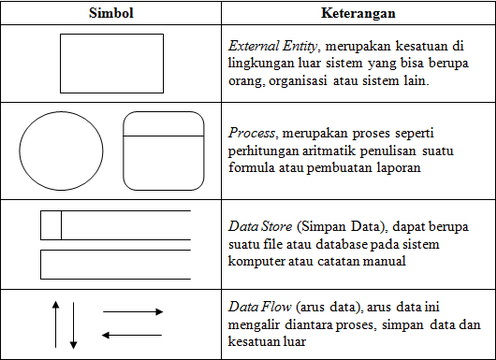
\includegraphics[scale=0.9]{figure/dfd.jpg}
    \caption{\textit{Simbol DFD}}
    \label{gambar 3}
\end{figure}


 
\chapter{Analisis}
\section{Analisis Sistem}
Analisis sistem dapat didefinisikan sebagai penguraian dari suatu sistem informasi yang utuh kedalam bagian-bagian komponennya dengan maksud untuk mengidentifikasi dan mengevaluasi urutan algoritma dan fungsi-fungsi dalam sistem yang berjalan. Pada bagian ini, akan dibahas mengenai Analisis Aplikasi Downloader Mp4 Youtube akan digambarkan dalam bentuk \textit{flowmap} dan \textit{data flow diagram}.

\subsection{Analisis Sistem yang sedang berjalan}
Untuk gambaran sistem yang berjalan dalam aplikasi Downloader Mp4 Youtube adalah proses dimana informasi yang terdapat pada aplikasi dapat digunakan sebagai media mendownload video yang terdapat pada aplikasi Downloader Mp4 Youtube. 

\subsubsection{Analisis Prosedur (Flowmap)}
Prosedurnya di awali dari user membuka aplikasi website Downloader Mp4 Youtube {(savefrom.net)}kemudian membuka Youtube sebagai media penyedia video .

\begin{enumerate}
    \item Mulai.
    \item Mambuka website Youtube lalu cari video yang di inginkan kemudian copy URL video Youtube tersebut.
    \item Pada tab lain buka website aplikasi Downloader Mp4 Youtube {(savefrom.net)}.
    \item Kemudian tempel url video Youtube pada aplikasi Downloader Mp4 Youtube {(savefrom.net)}.
    \item kemudian anda dapat memilih kulitas unduhan seperti Mp4 serta WEBM.
    \item Jika sudah menentukan kualiatas, anda dapat menekan tombol download 
    \item Setelah itu User dapat menerima notifikasi serta tujuan penyimpanan download video atau musik.
    \item Selesai.
\end{enumerate}

\begin{figure}[!htbp]
    \centering
    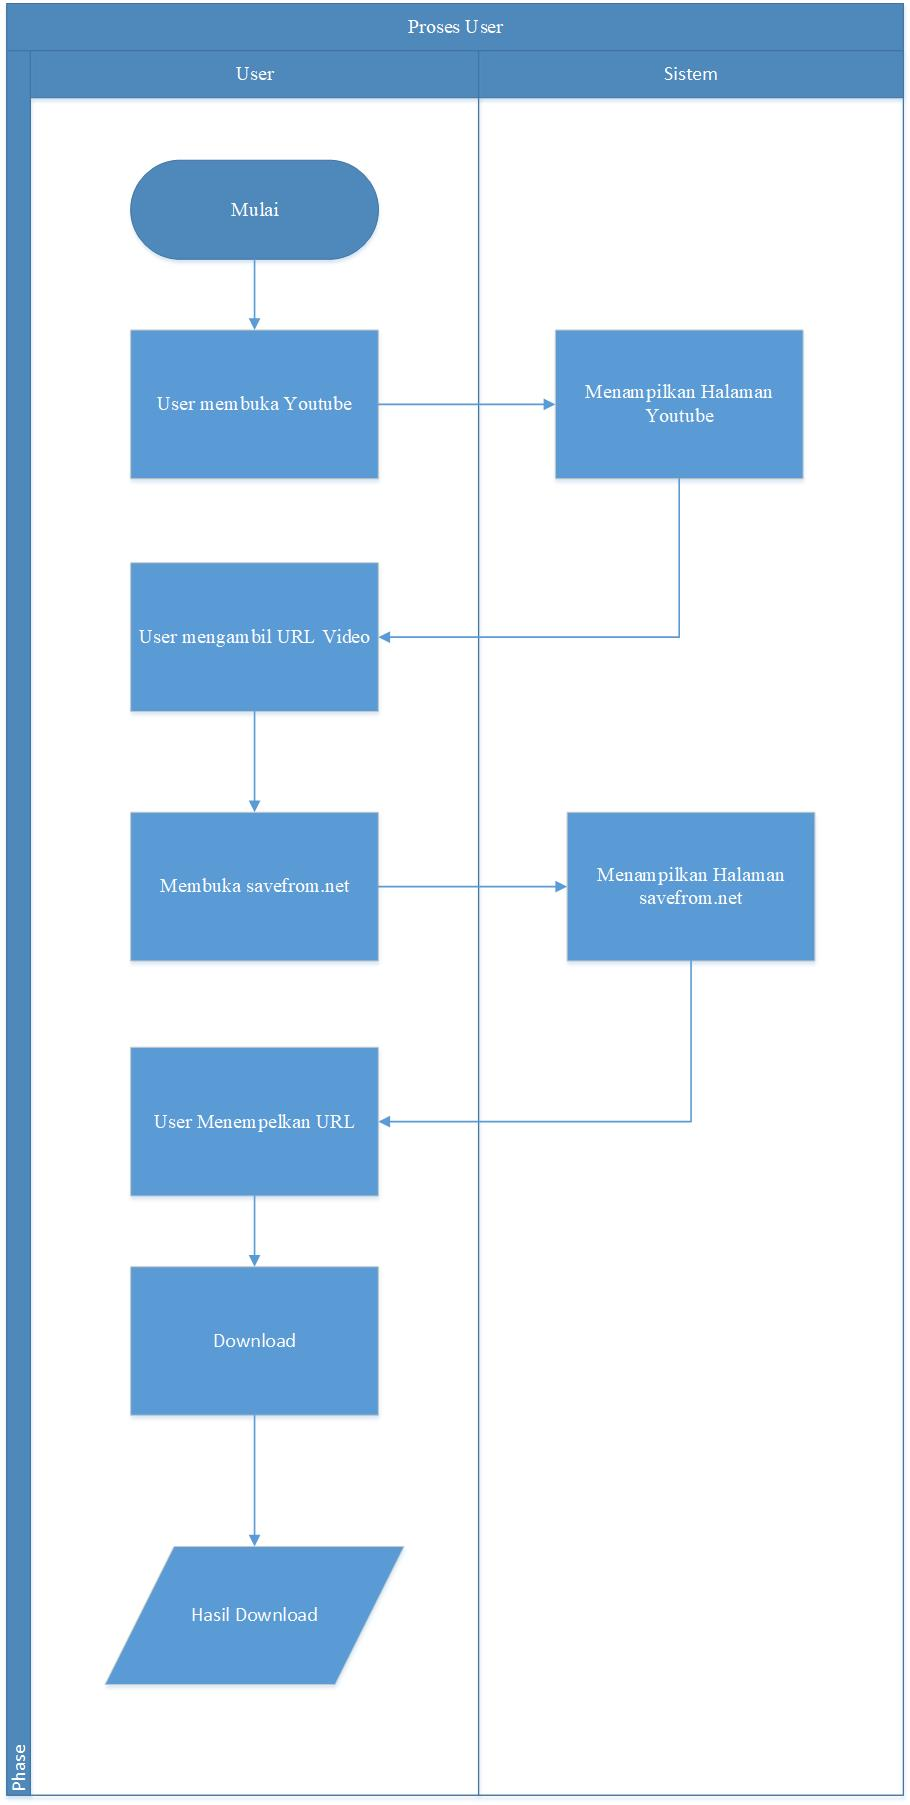
\includegraphics[scale=0.6]{figure/Drawing2.jpg}
    \caption{\textit{flowmap Mp4 youtube yang berjalan }}
    \label{gambar 1}
\end{figure}

\subsection{Kebutuhan Perangkat lunak }
Kebutuhan perangkat lunak dimaksud disini adalah berupa software pendukung yang bisa digunakan pada proses berjalannya aplikasi Downloader Mp4 Youtube :
\begin{enumerate}
    \item Anaconda 3 2019.07 64-bit
    \item Spyder 3.3.6 64-bit
    \item Python 3.7.3 64-bit
    \item firefox quantum 69.0.1 64-bit
\end{enumerate}

\section{Analisis DFD}
\subsection{Data Flow Diagram}
Data Flow Diagram adalah salah satu cara untuk menjelaskan sistem secara logika bagaimana arus data yang berjalan dalam sistem tersebut.

\subsubsection{Data Flow Diagram Level 0}
Data Flow Diagram level 0 merupakan penjelasan dasar arus informasi dari Youtube dan aplikasi Downloader Mp4 {(savefrom.net)}.

\begin{figure}[!htbp]
    \centering
    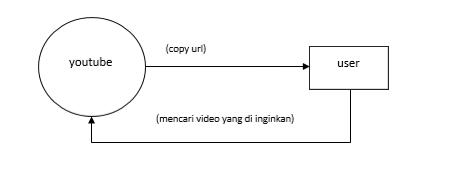
\includegraphics[scale=1]{figure/youtube.jpeg}
    \caption{\textit{DFD level 0 dari youtube}}
    \label{gambar 1}
\end{figure}


Data Flow Diagram level 0 pada youtube, mencakup:
\begin{enumerate}
    \item Berisi 2 Entitas, yaitu user dan admin.
    \item Kemudian berisi 1 Proses, dari Youtube.
\end{enumerate}

\begin{figure}[!htbp]
    \centering
    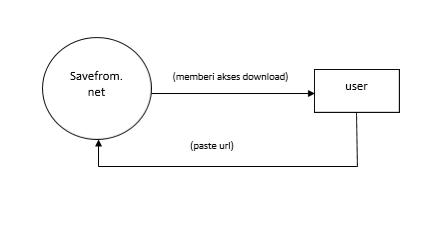
\includegraphics[scale=1]{figure/savefrom.jpeg}
    \caption{\textit{DFD level 0 dari savefrom.net}}
    \label{gambar 1}
\end{figure}
\vspace{1cm}
Data Flow Diagram level 0 pada aplikasi savefrom.net, mencakup:
\begin{enumerate}
    \item Berisi 2 Entitas, yaitu user dan admin.
    \item Kemudian berisi 1 Proses, yaitu aplikasi Downloader Mp4 Youtube.
\end{enumerate}

\vspace{8cm}

\subsection{Spesifikasi Tabel}
\subsubsection{Spesifikasi Proses DFD Level 0}

Berikut spesifikasi proses DFD level 0 pada youtube dan savefrom.net terdapat  pada tabel \ref{tableSpec1}

\begin{table}[!htbp]
\centering
\caption{Tabel Spesifikasi}
\label{tableSpec1}
\begin{tabular}{|l|l|l|l|l|}
\hline
No & Proses & Masukan & Keluaran & Logika Proses \\
\hline

 & & & & \textit{Begin if}\\
 & & & & jika judul di: \\
 & & & & \textit{input} maka muncul  \\
 & & & & video \\
 & & \textit{input} judul& menampilkan \\
1 &  Youtube & video & video & \textit{else if} \\
 & & & dan url& judul = valid \\
 & & & & \textit{then} \\
 & & & & tampilkan video dan url \\
 & & & & \textit{Endif} \\
\hline

 & & & & \textit{Begin if}\\
 & & & & jika url: \\
 & & & & terbaca maka muncul  \\
 & & & & video \\
 & & \textit{copy link} & menampilkan  & hasil dari Youtube \\
1 &  Aplikasi savefrom.net &url& link & \textit{else if} \\
 & & & download& url = valid \\
 & & & & \textit{then} \\
 & & & & tampilkan menu download \\
 & & & & \textit{Endif} \\
\hline

\end{tabular}
\end{table}

\subsection{Testing}
Antar muka atau \textit{User Interface} (UI) adalah cara sebuah program berinteraksi langsung dengan pengguna dengan kata lain segala sesuatu dirancang menjadi sebuah perangkat informasi sehingga pengguna dapat lebih mudah melakukan interaksi dengan program. Dalam merancang sebuah user interface kita harus memperhatikan beberapa hal:
\begin{enumerate}
    \item User Interface yang sederhana, maksudnya didalam aplikasi tersebut tidak ada elemen fungsi yang kira kiranya tidak diperlukan dan hanya terdapat elemen yang dibutuhkan oleh pengguna.
    \item User Interface juga dibentuk sesuai siapa pengguna aplikasi tersebut. Sehingga dapat menyesuaikan kemampuan dan pengalaman user dalam berinteraksi.
    \item Penempatan layout agar tidak memepersulit pengguna dalam menggunakan sebuah aplikasi.
 
\end{enumerate} 
\subsubsection{Perancangan Antar Muka yang Sedang Berjalan}
Antar Muka yang sedang berjalan dalam aplikasi Downloader Mp4 adalah bagaimana alur proses dari pembukaan Youtube sampai download video pada aplikasi savefrom.net.

\begin{figure}[!htbp]
    \centering
    
\includegraphics[scale=1.5]{figure/CMD.png}
    \caption{Proses pada cmd }
    \label{gambar 1}
\end{figure}

\begin{figure}[!htbp]
    \centering
    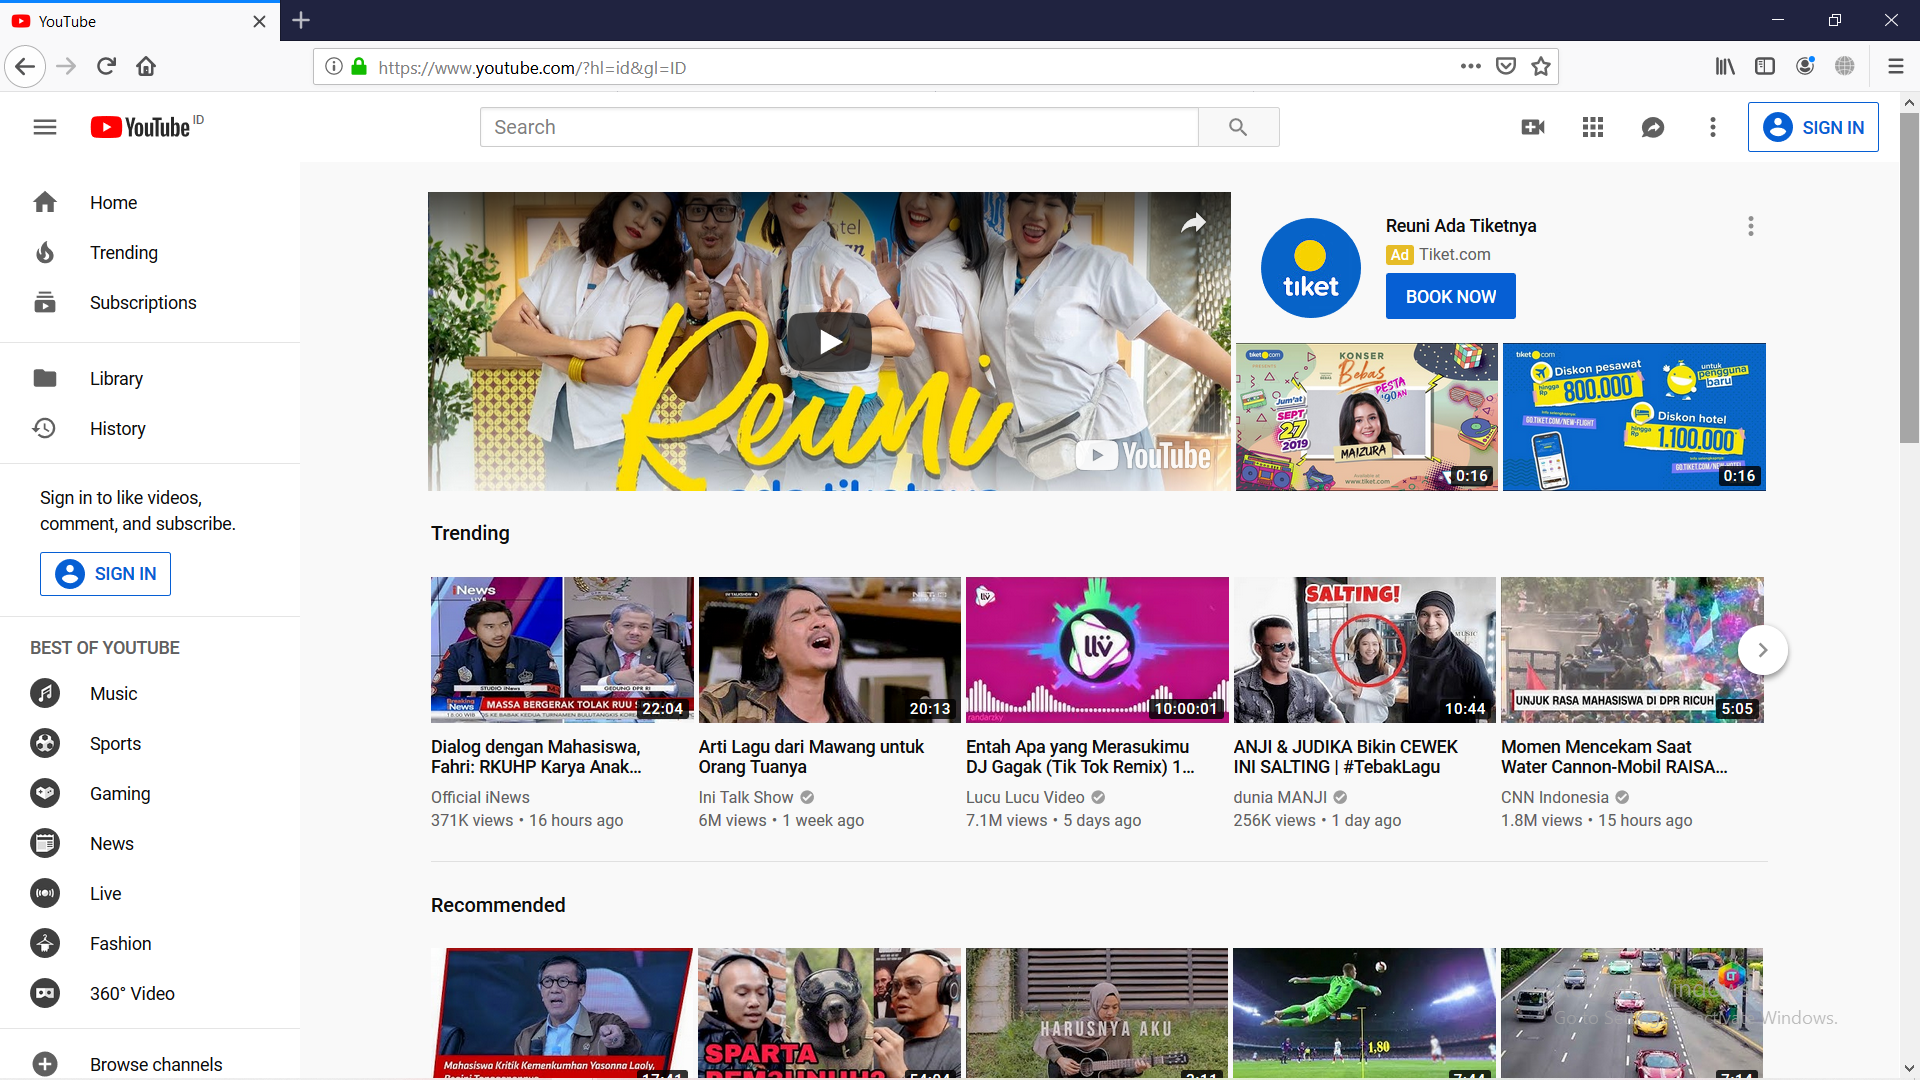
\includegraphics[scale=0.4]{figure/Antarmuka/1.png}
    \caption{ Proses pada Pembukaan youtube}
    \label{gambar 1}
\end{figure}

\begin{figure}[!htbp]
    \centering
    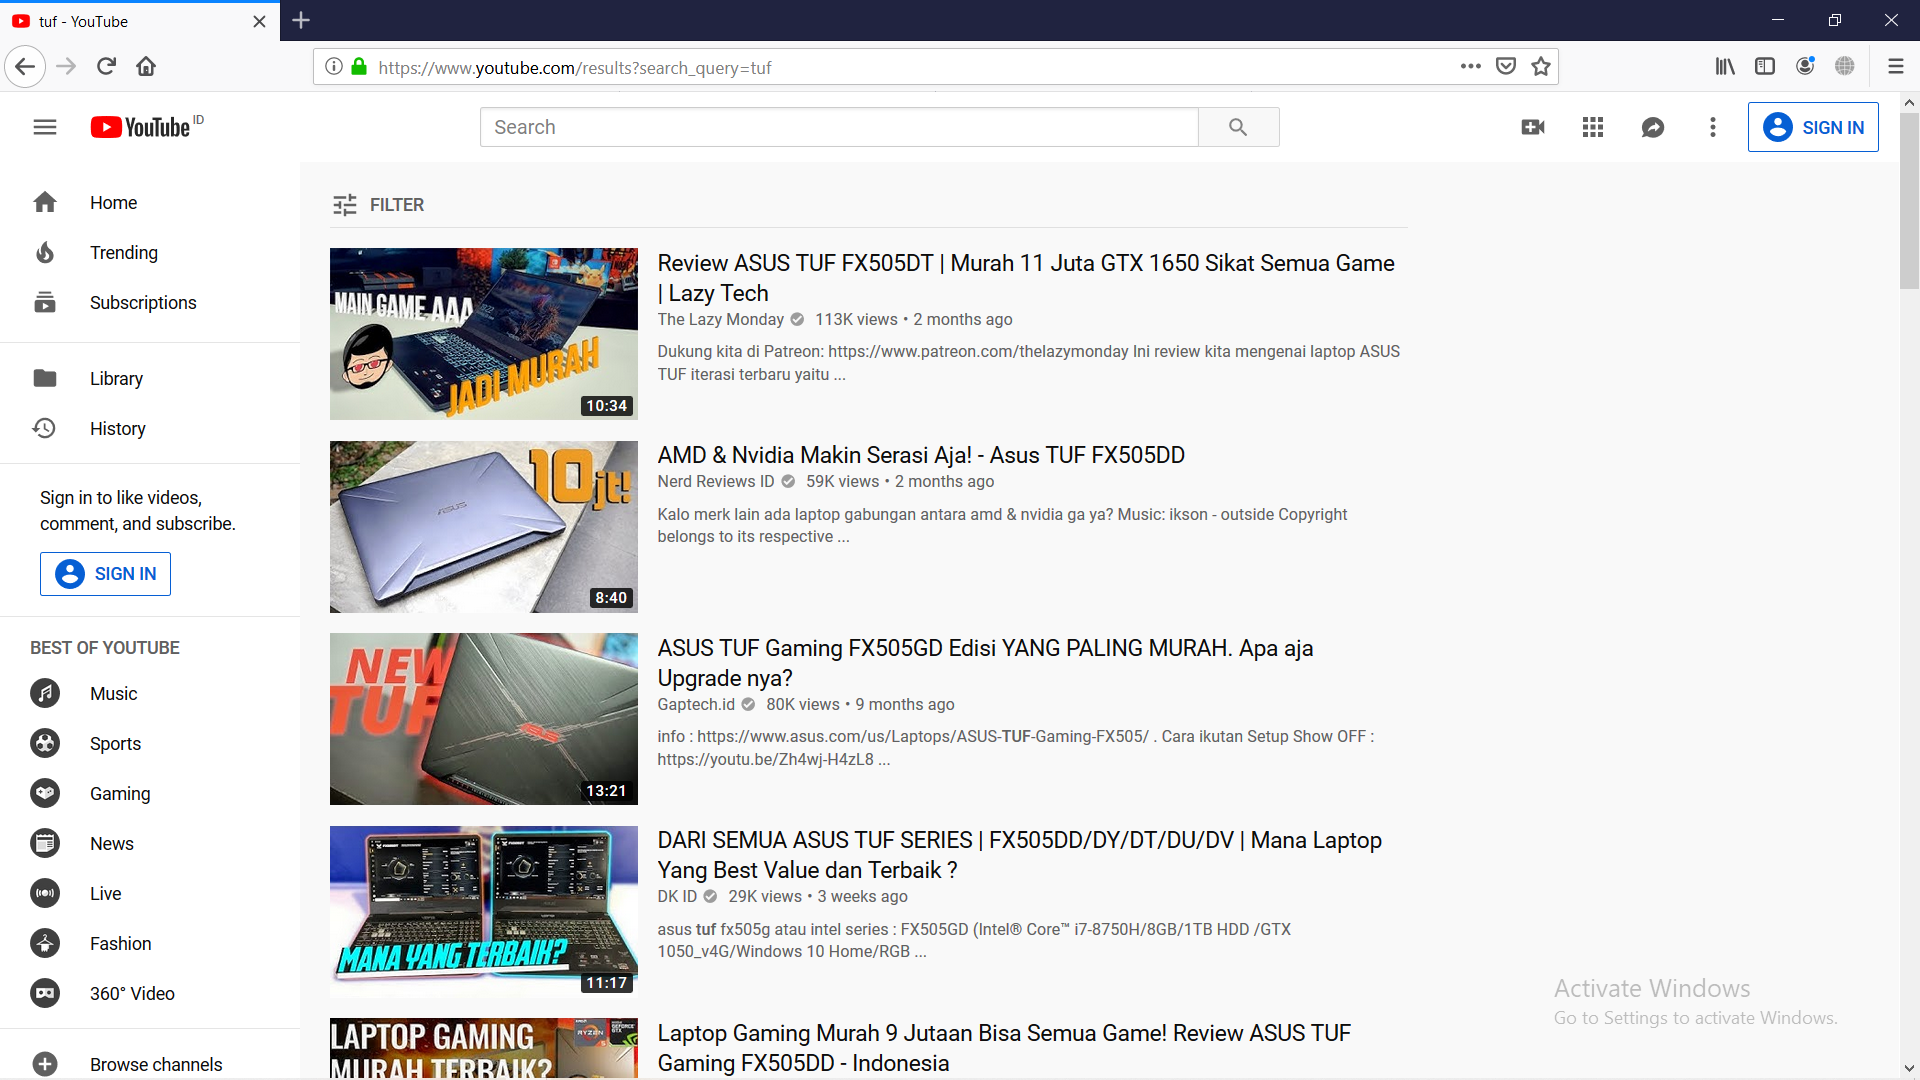
\includegraphics[scale=0.4]{figure/Antarmuka/2.png}
    \caption{ Proses pada saat mencari video}
    \label{gambar 1}
\end{figure}

\begin{figure}[!htbp]
    \centering
    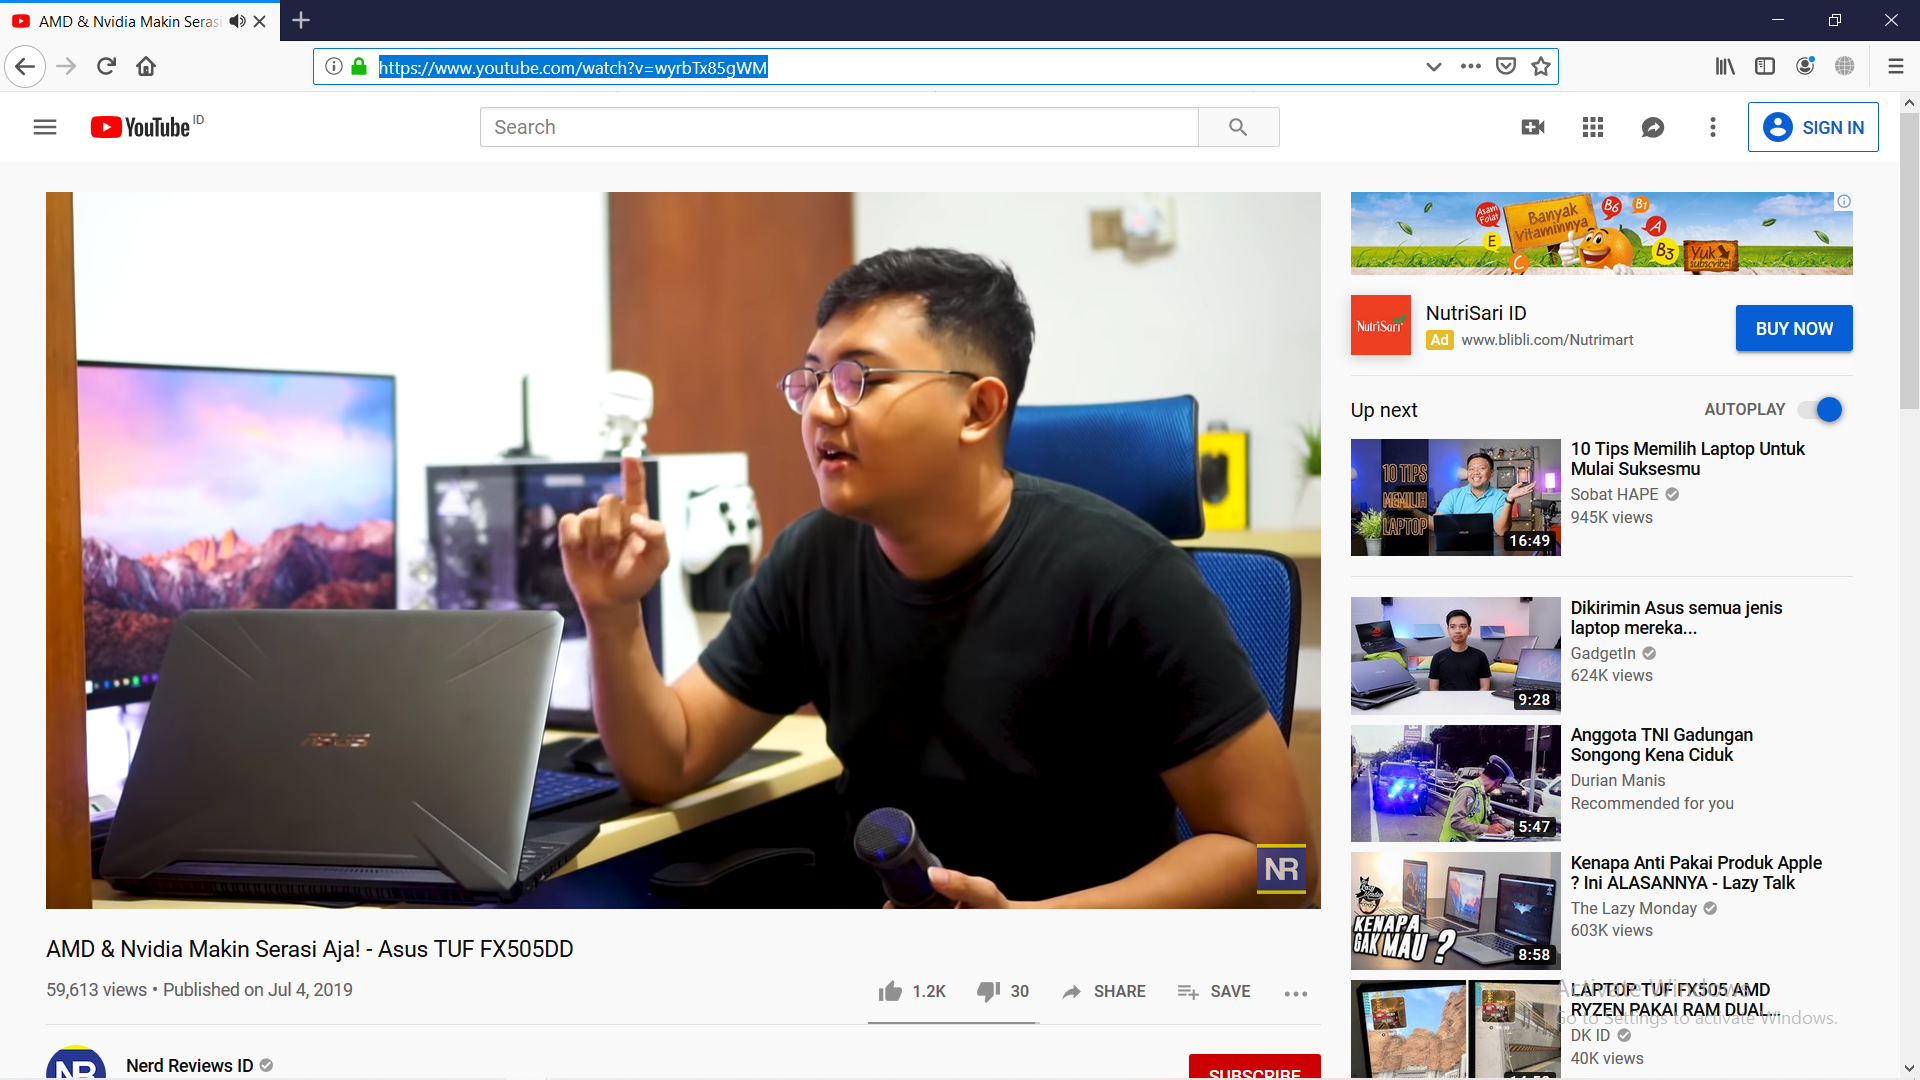
\includegraphics[scale=0.4]{figure/Antarmuka/3.png}
    \caption{ Proses saat mengambil Url video}
    \label{gambar 1}
\end{figure}

\begin{figure}[!htbp]
    \centering
    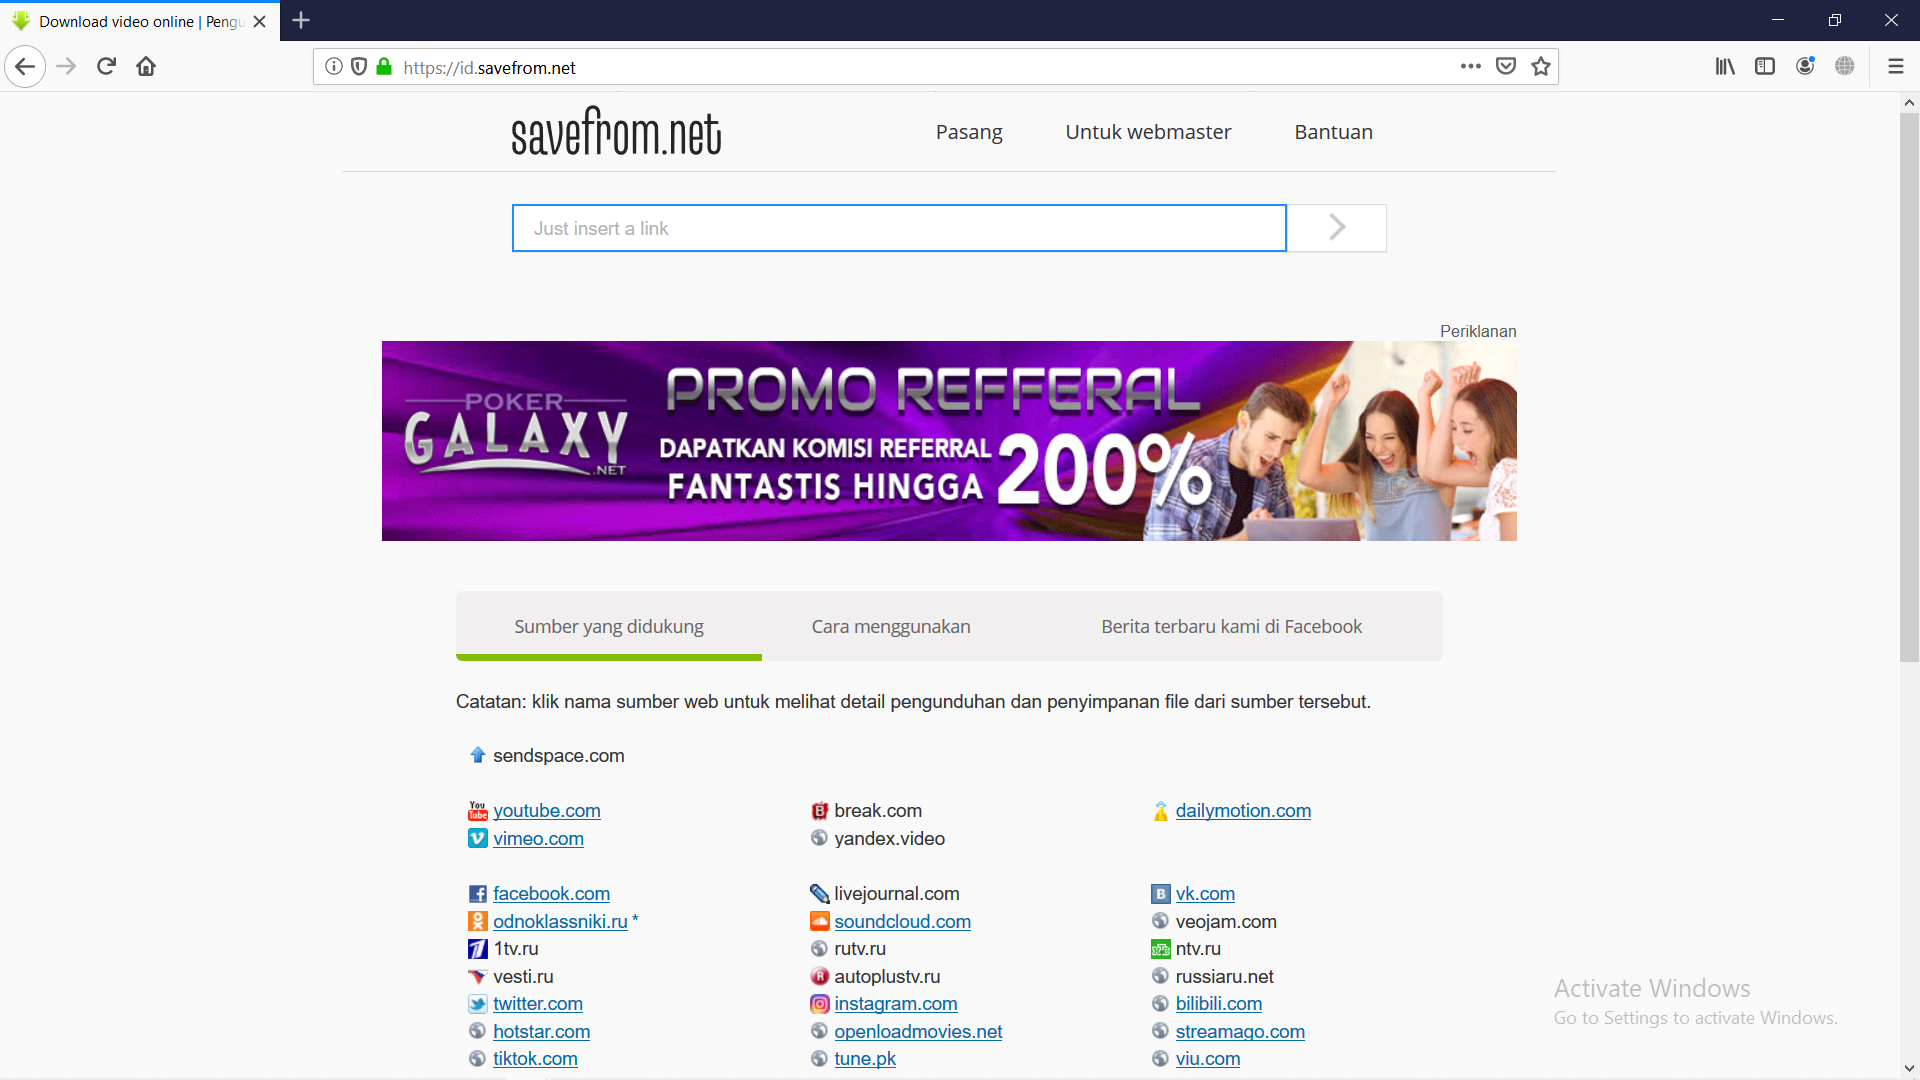
\includegraphics[scale=0.4]{figure/Antarmuka/4.png}
    \caption{ Proses saat membuka savefrom.net}
    \label{gambar 1}
\end{figure}


\begin{figure}[!htbp]
    \centering
    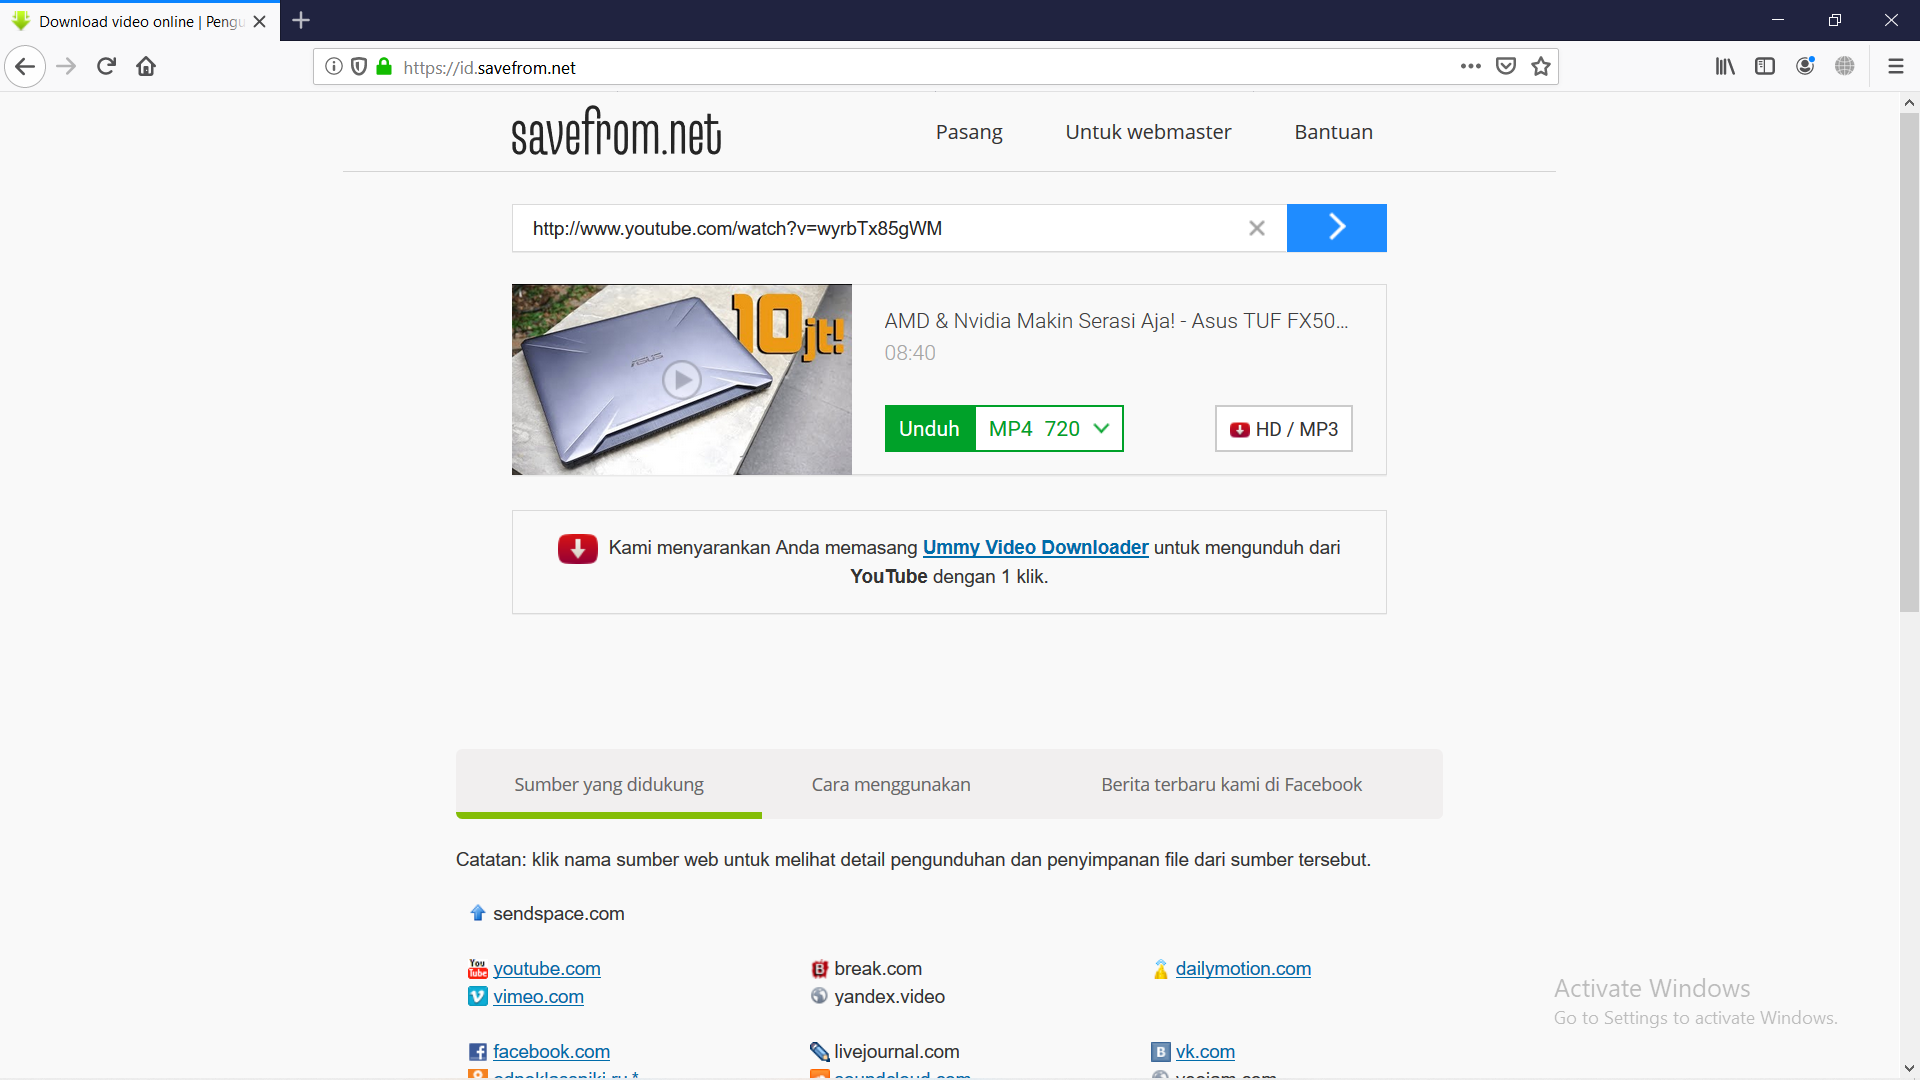
\includegraphics[scale=0.4]{figure/Antarmuka/5.png}
    \caption{Proses saat copy url pada savefrom.net}
    \label{gambar 1}
\end{figure}

\begin{figure}[!htbp]
    \centering
    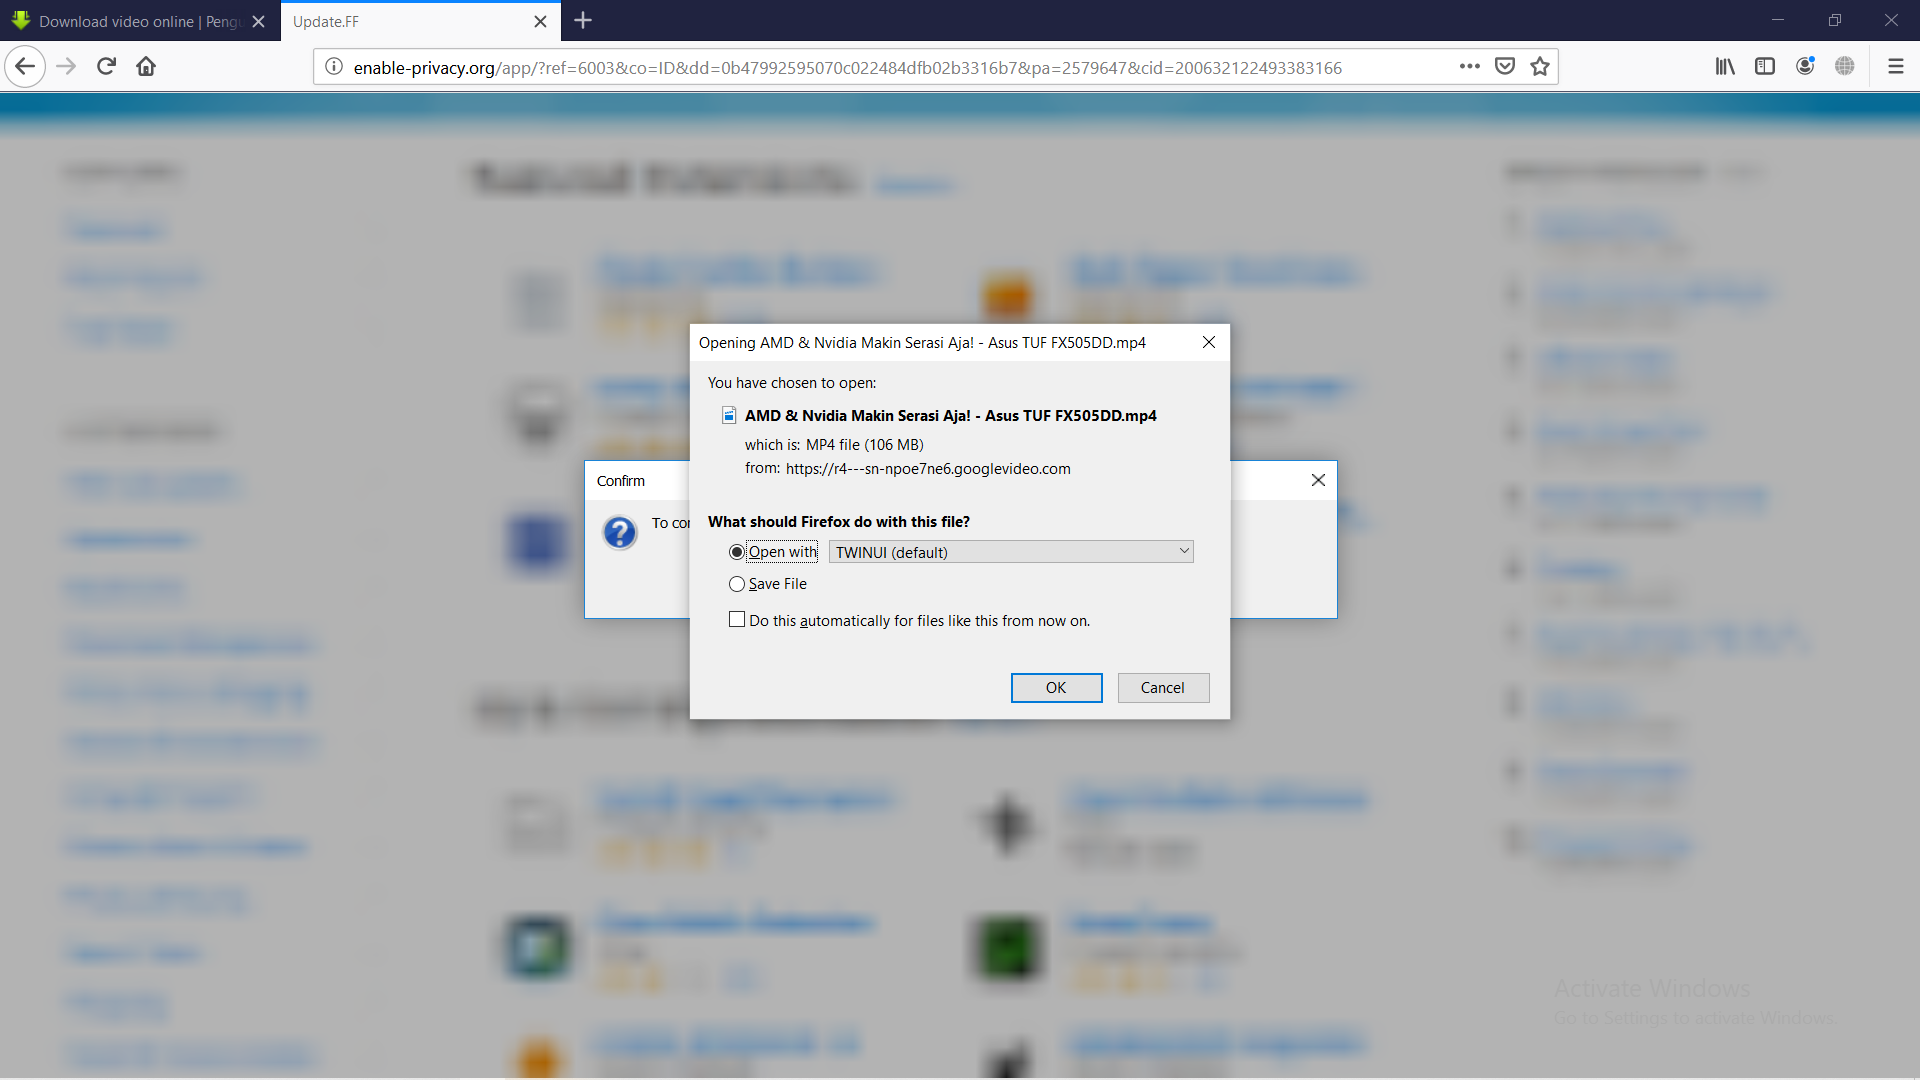
\includegraphics[scale=0.4]{figure/Antarmuka/9.png}
    \caption{ Proses saat video bisa di download}
    \label{gambar 1}
\end{figure} 
\chapter{Implementasi}
\section{Lingkungan Implementasi}
Sesudah menyelesaikan proses analisis, proses yang dilakukan pada tahap selanjutnya adalah perancanagan program dimana semua dijalankan secara otomatis pada tahap mencari dan mendownload.


\subsection{Menggunakan Selenium}
    Pada tahap ini bagaimana menjalannkan progran otomatis dengan web testing menggunakan Python dan menggunkan IDE Spyder. Disini Program Menjalankan Printah otomatis Membuka,mengambil url sampai muncul nya akses download secara otomatis, dengan codingan yaitu: :

\begin{enumerate}
    \item search=('tuf') :
    merupakan variable yang menampung nilai string dimana Tuf adalah judul video yang dicari
    \item youtube = webdriver.Firefox() :
    merupakan variable yang akan memanggil webdriver Firefox
    \item youtube.get('https://www.youtube.com/') :
    variable yang berisikan alamat url dari youtube 
    \item youtube.get('https://www.youtube.com/results?search-query= '+ search) :
    varible yang akan memanggil youtube serta penambahan variable dari search. fungsi dari search inilah yang memberikan judul dari video yang akan di cari
    \item youtube.get('https://en.savefrom.net/') :
    variable yang memanggil savefrom.net melalui url
    \item youtube.find\_element\_by\_id('sf-url').send\_keys('https://www.youtube.com/watch
    ?v=wyrbTx85gWM') :
    codingan ini berfungsi sebagai media tempat paste url dari youtube dan membeberikan url video
    \item youtube.find\_element|\_by\_xpath('//*[@id="sf-submit"]').click() :
    codingan ini berfungsi memunculjkan tampilan download yang ada pada savefrom.net.
    \item sleep(3) : memberikan jeda waktu 3 detik untuk menampilakan tombol download 
    \item youtube.find\_element\_by\_xpath('/html/body/div/div[1]/div[3]/div[4]/div/div[1]
    /div[2]/div[2]/div[1]/a').click() : codingan yang berfungsi  untuk menekan tombol download pada savefrom.net secara otomatis.
\end{enumerate}

\subsection{Cara pengambilan Element pada Web }
    Pada Tahapan ini akan diberitahu cara mengambil element sebagi berikut:

\begin{enumerate}
    \item Kita ambil contoh website tersebut adalah savefrom.net. Kita akan Inspect kode Program.
\begin{figure}[!htbp]
    \centering
    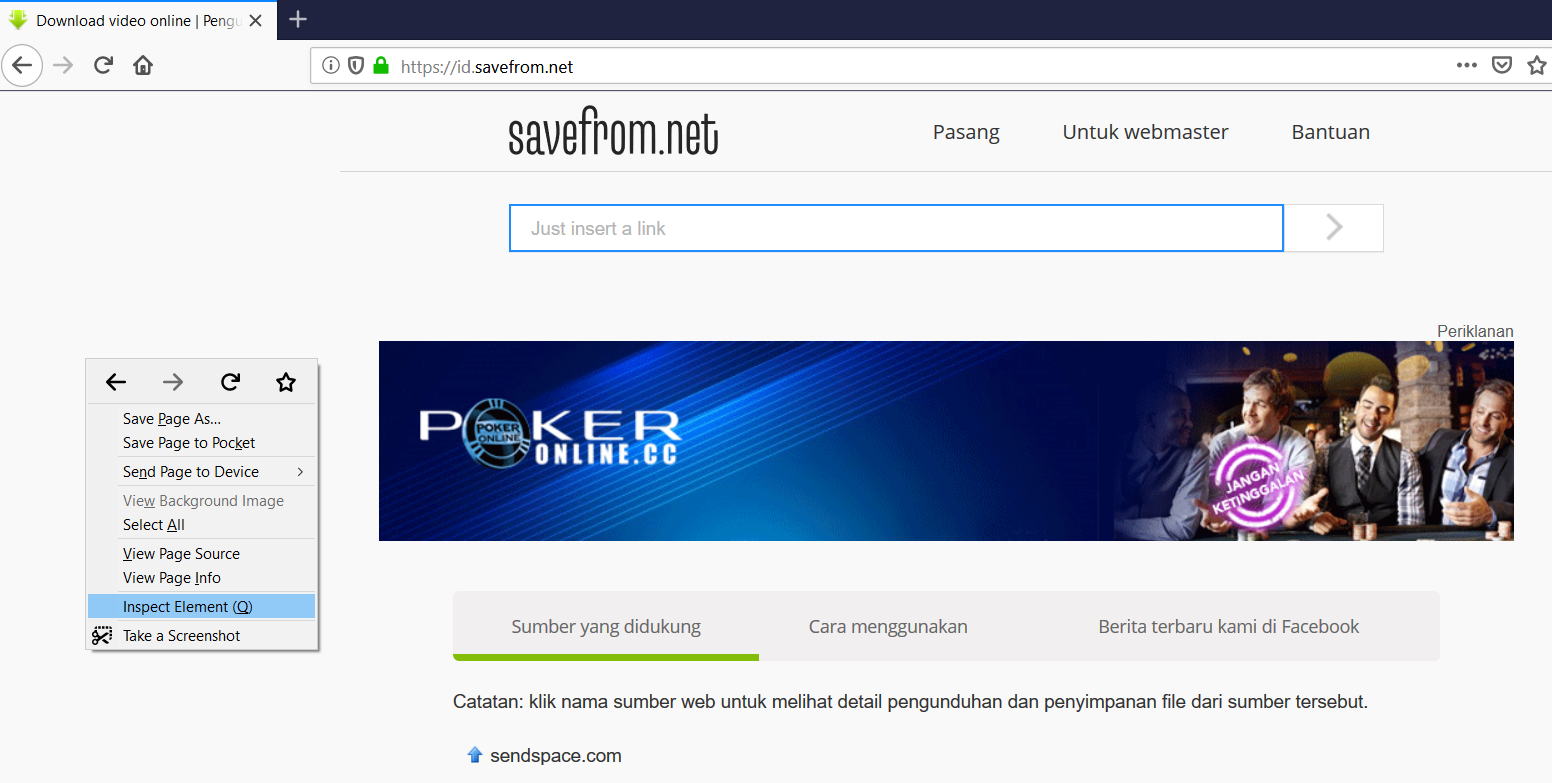
\includegraphics[scale=0.3]{figure/inspect.png}
    \label{gambar 1}
\end{figure}
    \item Kemudian ketika menekan inspect maka akan muncul hasil dari inspect code program, kemudian klik kanan, kemudian pada menu copy klik xpath.
\begin{figure}[!htbp]
    \centering
    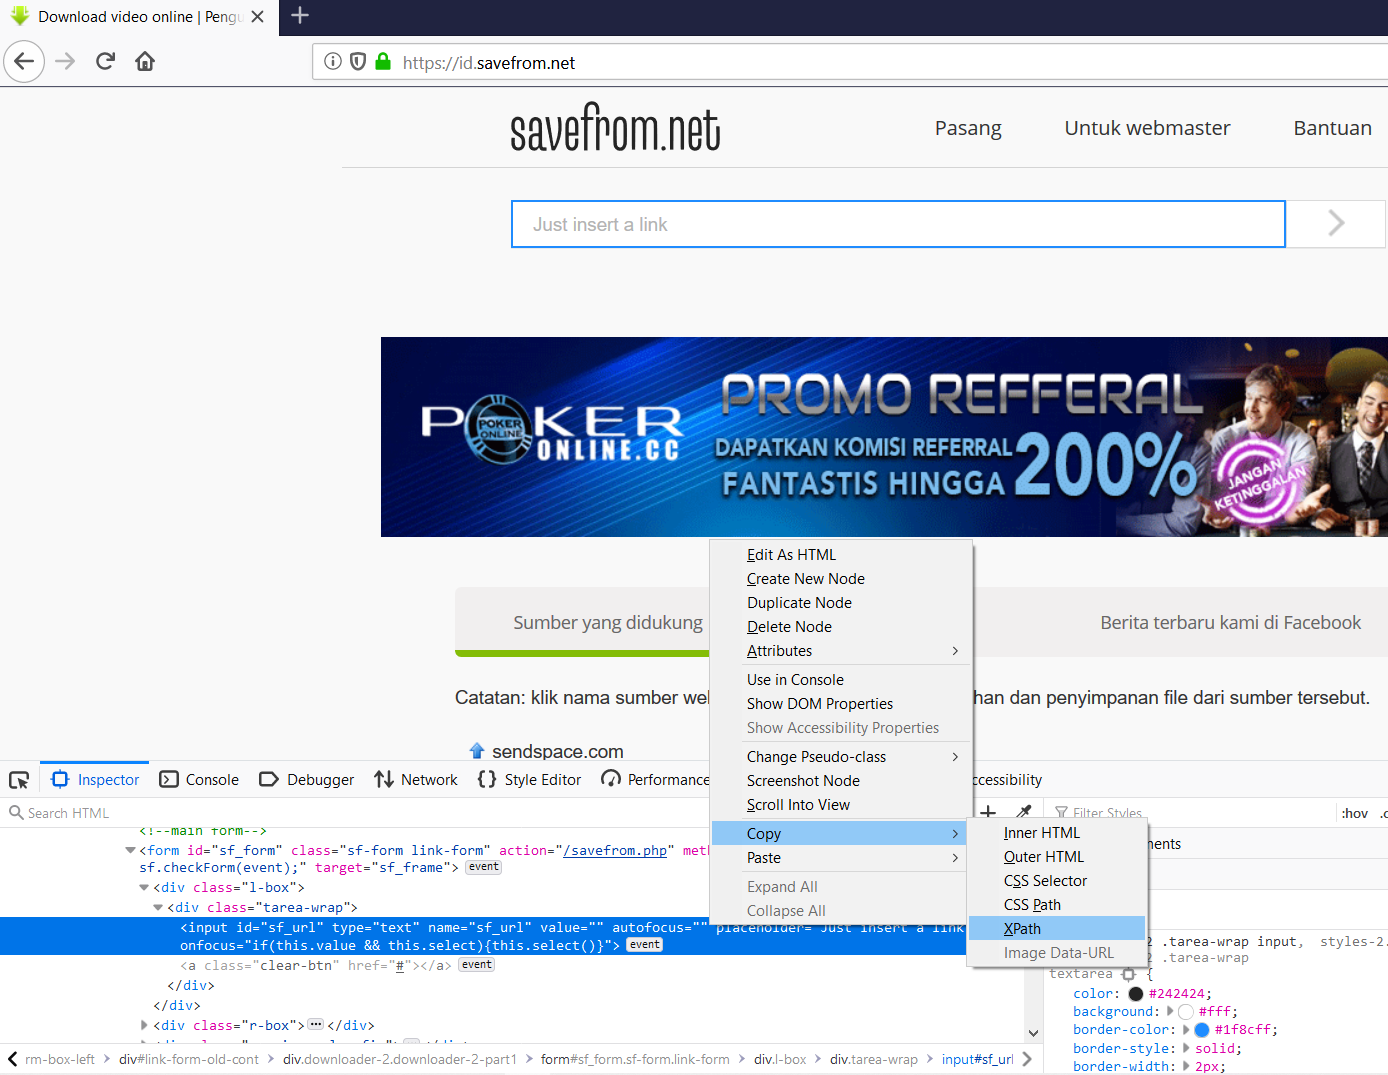
\includegraphics[scale=0.3]{figure/hasil1.png}
    \label{gambar 4}
\end{figure}
\end{enumerate}
  
\section{Pengujian dan Hasil Pengujian}
\subsection{Pengujian}
Berikut ini ada beberapa tahapan pengujian jalannya pengoperasian download secara otomotis 

\begin{enumerate}
    \item Kita menggunakan find\_element sebagai Pemberikan text secara otomatis. Saat  Di run hasil pada menu search pada youtube tidak muncul text yang telah ditentukan. Dan pada Spyder {(unknown variant search)}
\begin{figure}[!htbp]
    \centering
    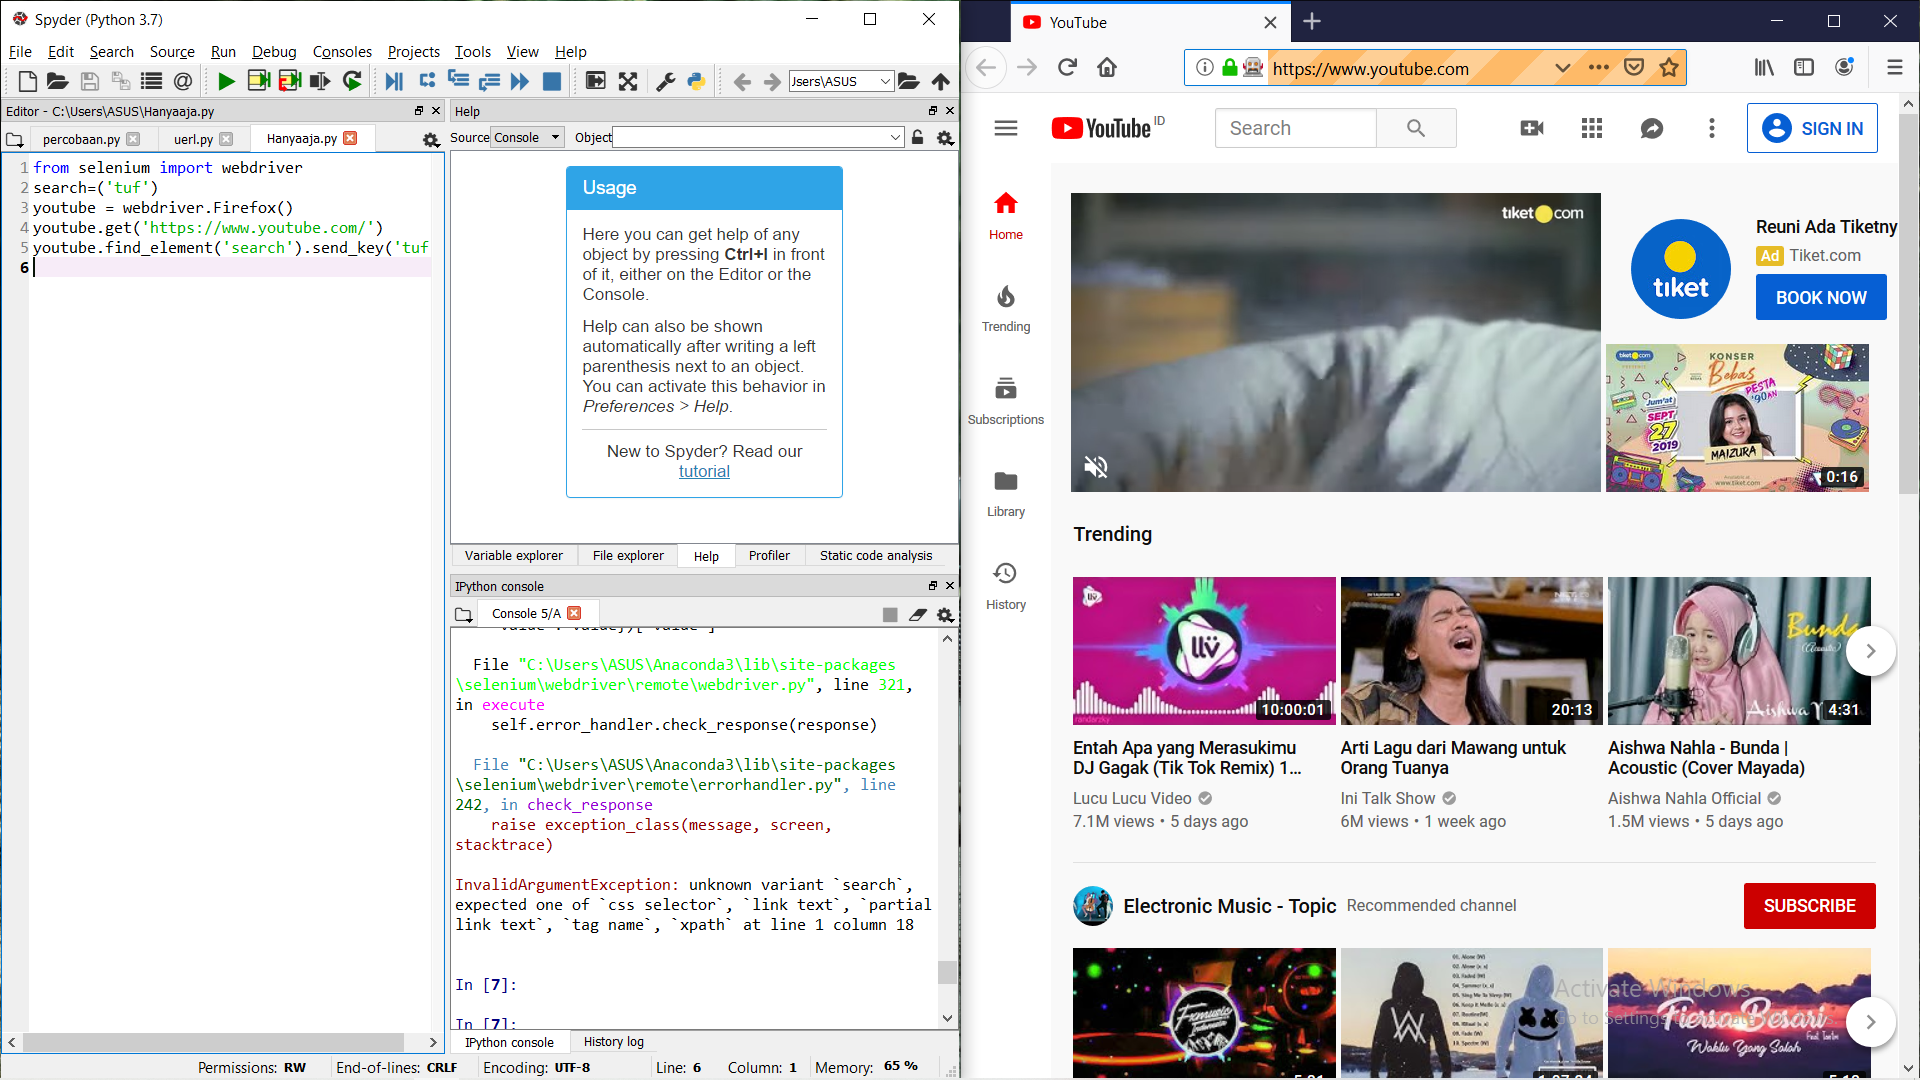
\includegraphics[scale=0.3]{figure/hasilTes/1.png}
    \label{gambar 1}
\end{figure}
\vspace{10cm}
    \item Kita menggunakan find\_element\_by\_class\_name sebagai Pemberikan text secara otomatis. Saat  Di run hasil pada menu search pada youtube tidak muncul text yang telah ditentukan. Dan pada Spyder {(unknown variant search)}
\begin{figure}[!htbp]
    \centering
    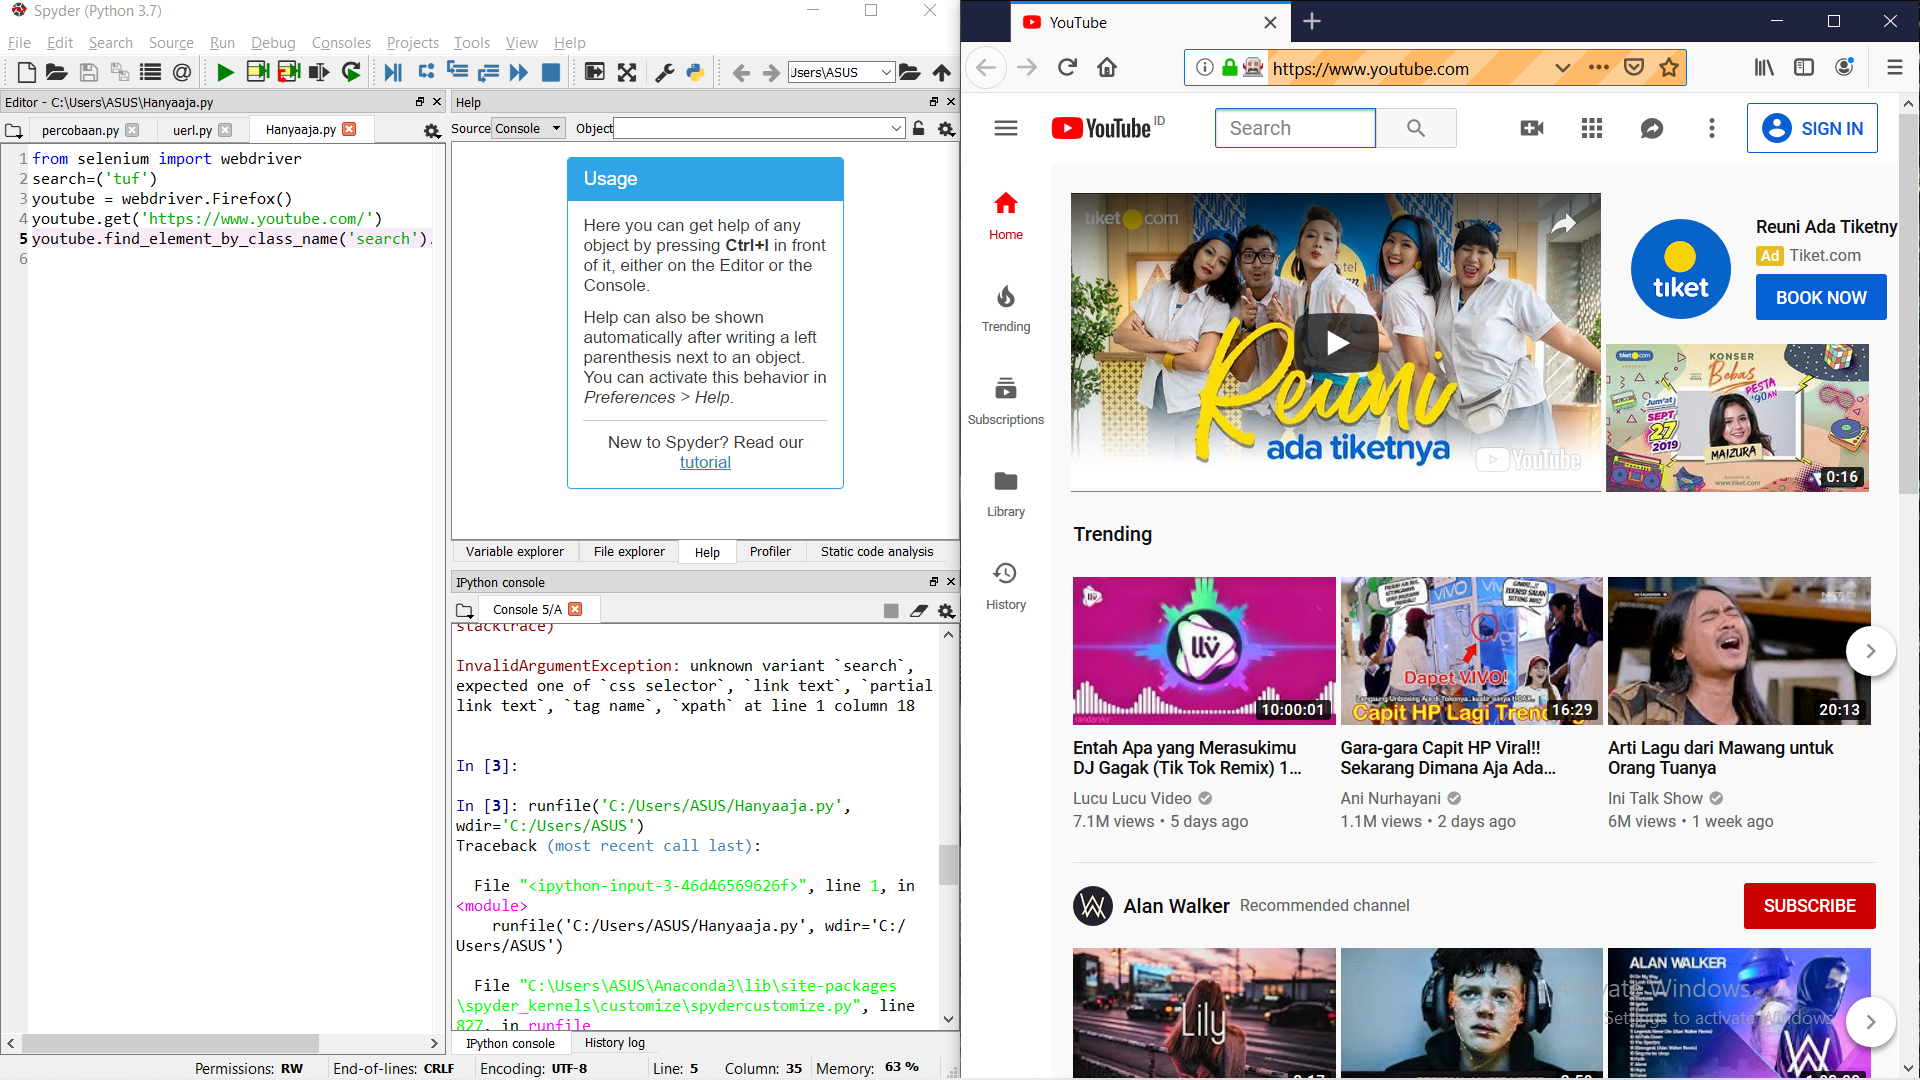
\includegraphics[scale=0.3]{figure/hasilTes/2.png}
    \label{gambar 1}
\end{figure}

     \item Kita menggunakan find\_element\_by\_id sebagai Pemberikan text secara otomatis. Saat  Di run hasil pada menu search pada youtube tidak muncul text yang telah ditentukan. Dan pada Spyder {(unable to locate search element)}
\begin{figure}[!htbp]
    \centering
    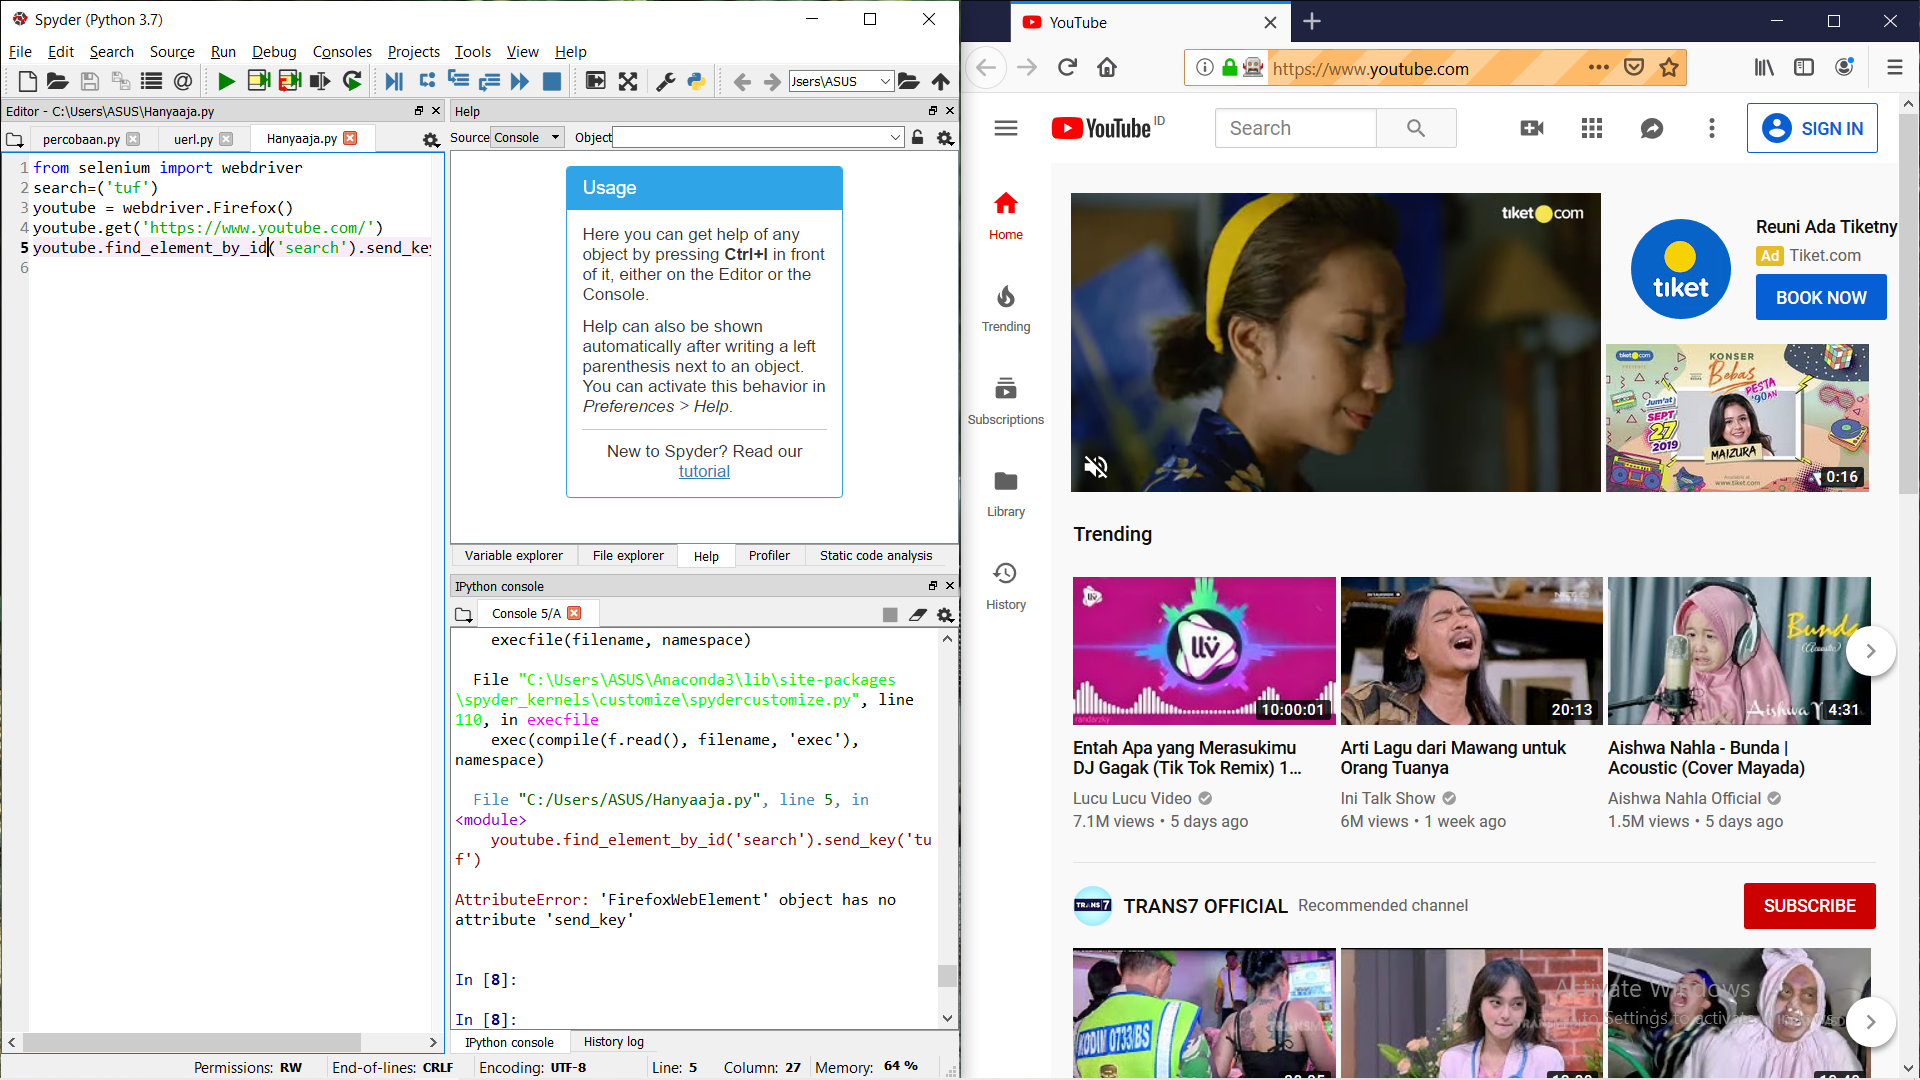
\includegraphics[scale=0.3]{figure/hasilTes/3.png}
    \label{gambar 1}
\end{figure}

    \item Kita menggunakan find\_element\_by\_link\_text sebagai Pemberikan text secara otomatis. Saat  Di run hasil pada menu search pada youtube tidak muncul text yang telah ditentukan. Dan pada Spyder {(unable to locate search element)}
\begin{figure}[!htbp]
    \centering
    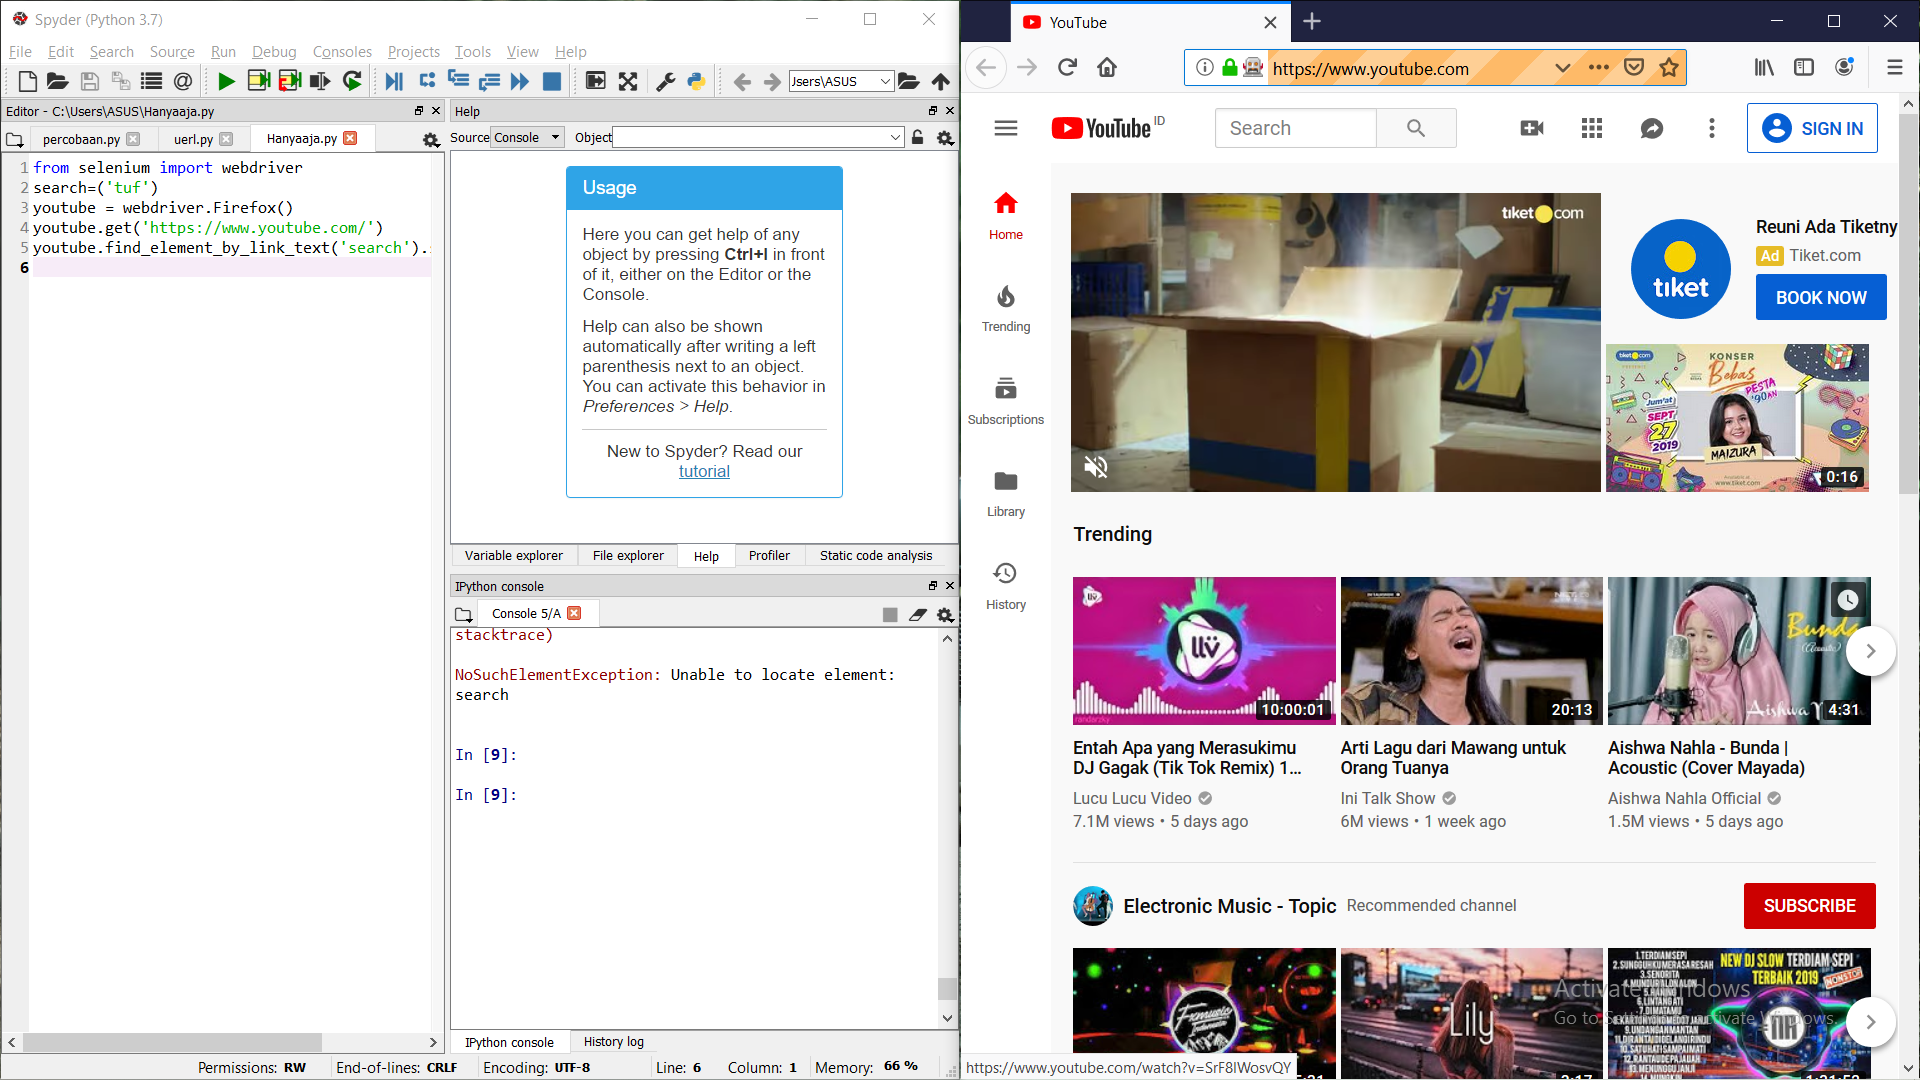
\includegraphics[scale=0.3]{figure/hasilTes/4.png}
    \label{gambar 1}
\end{figure}

    \item Kita menggunakan find\_element\_by\_name sebagai Pemberikan text secara otomatis. Saat  Di run hasil pada menu search pada youtube tidak muncul text yang telah ditentukan. Dan pada Spyder {(unable to locate name='search')}
\begin{figure}[!htbp]
    \centering
    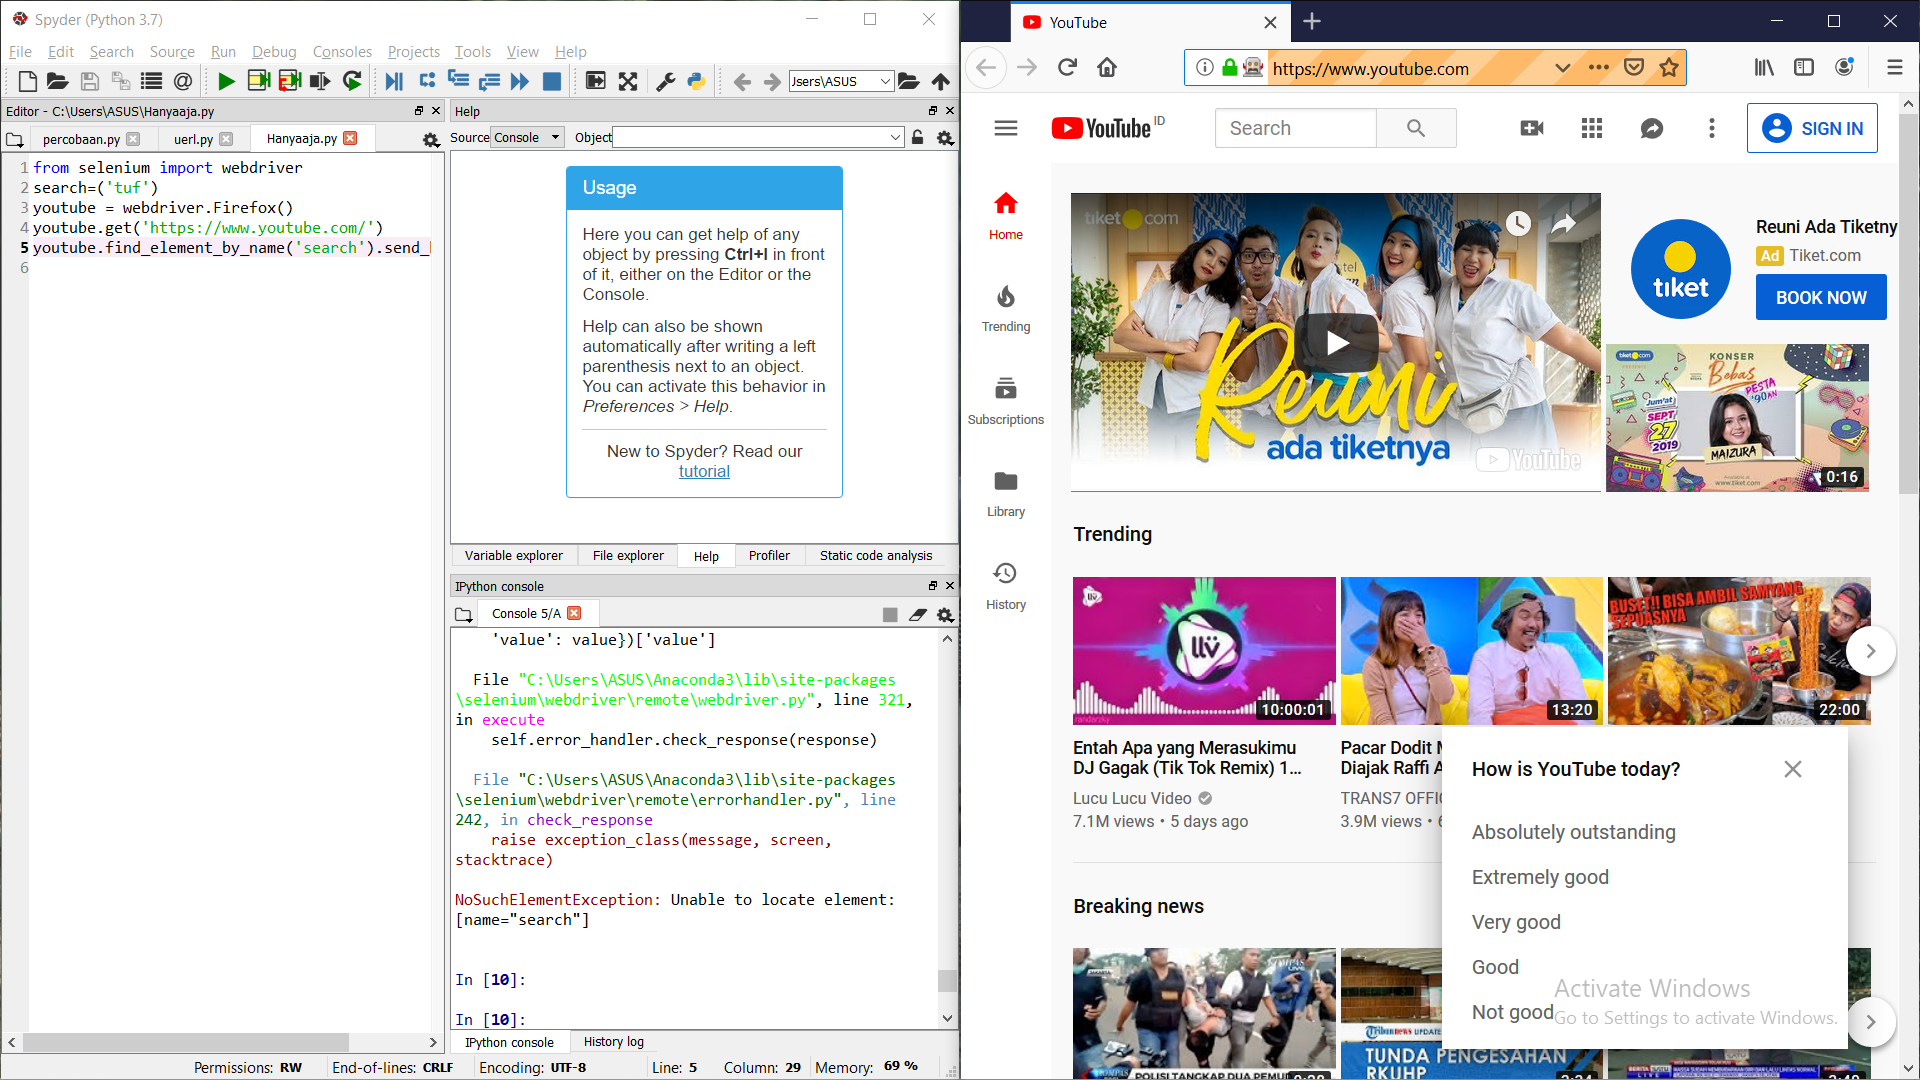
\includegraphics[scale=0.3]{figure/hasilTes/5.png}
    \label{gambar 1}
\end{figure}

    \item Kita menggunakan find\_element\_by\_partial\_link\_text sebagai Pemberikan text secara otomatis. Saat  Di run hasil pada menu search pada youtube tidak muncul text yang telah ditentukan. Dan pada Spyder {(unable to locate search element)}
\begin{figure}[!htbp]
    \centering
    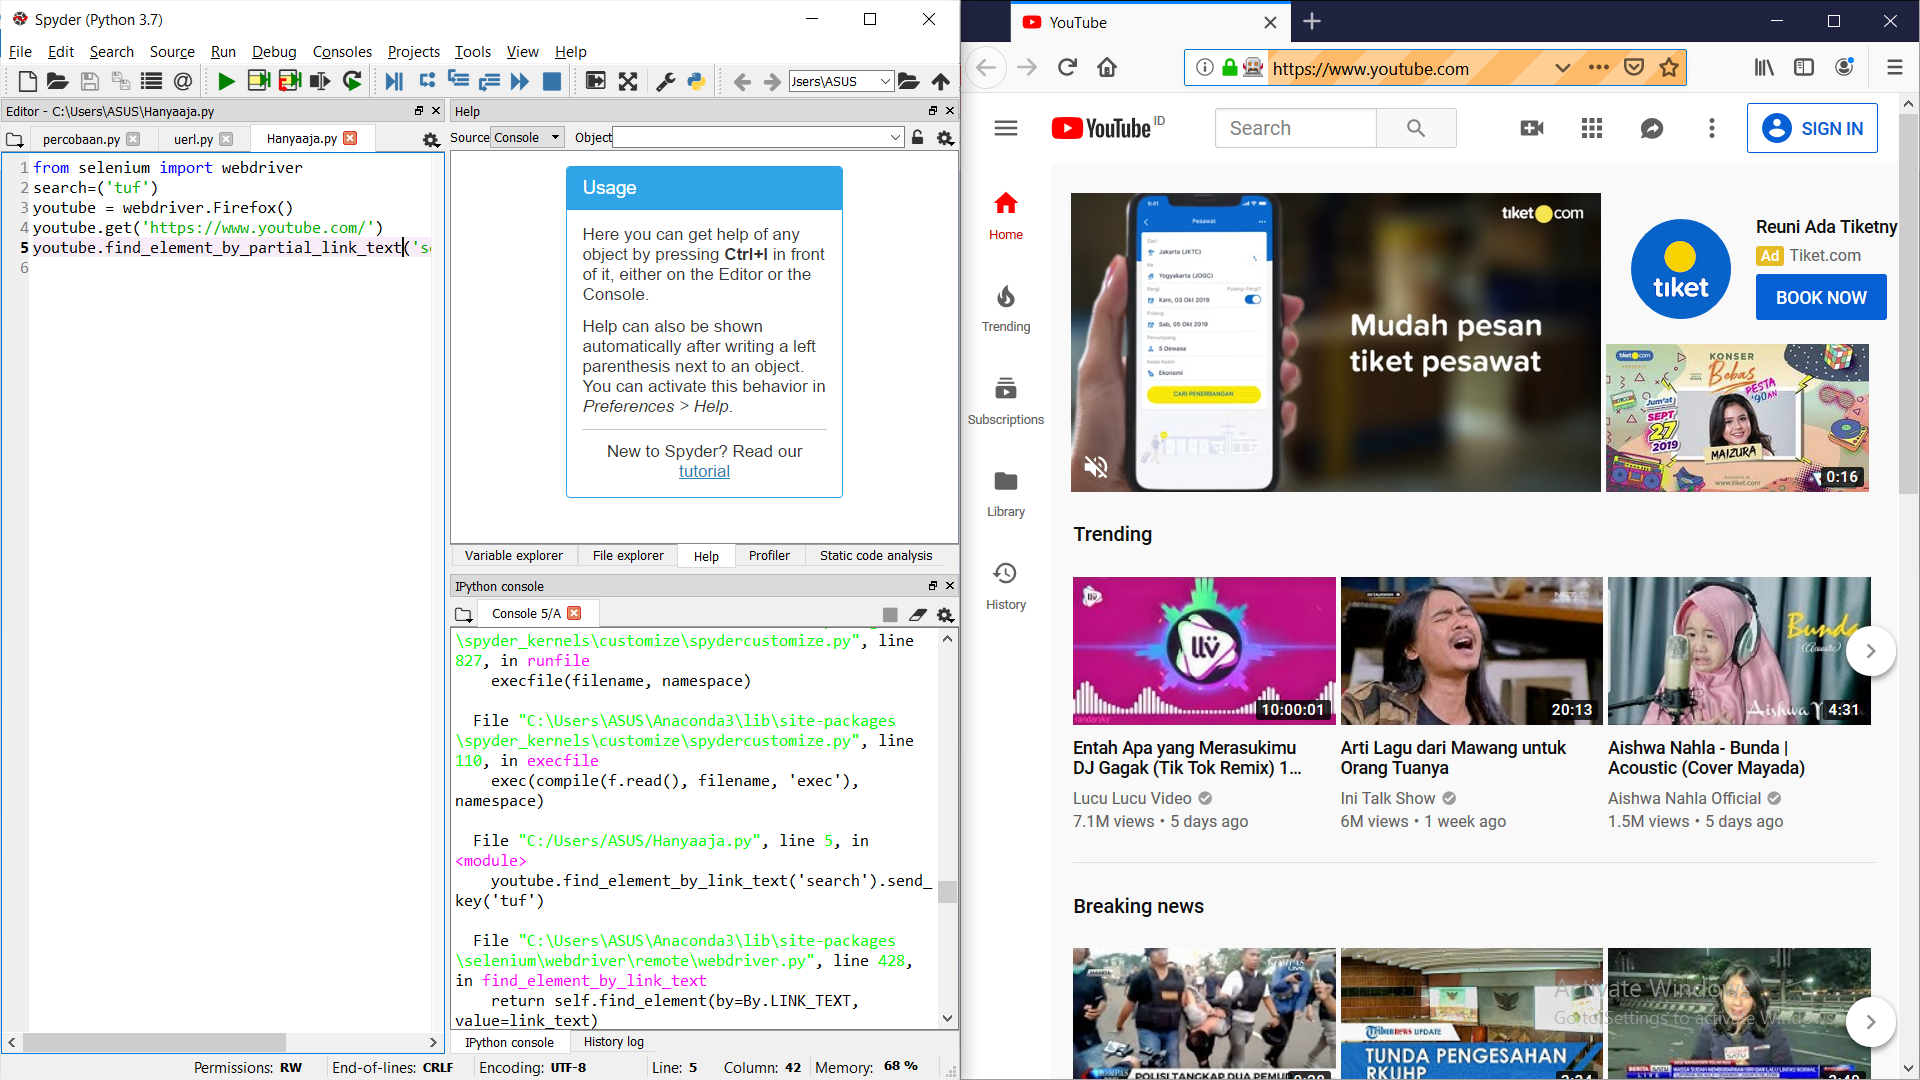
\includegraphics[scale=0.3]{figure/hasilTes/6.png}
    \label{gambar 1}
\end{figure}

\vspace{3cm}

    \item Kita menggunakan find\_element\_by\_tag\_name sebagai Pemberikan text secara otomatis. Saat  Di run hasil pada menu search pada youtube tidak muncul text yang telah ditentukan. Dan pada Spyder {(unable to locate search element)}
\begin{figure}[!htbp]
    \centering
    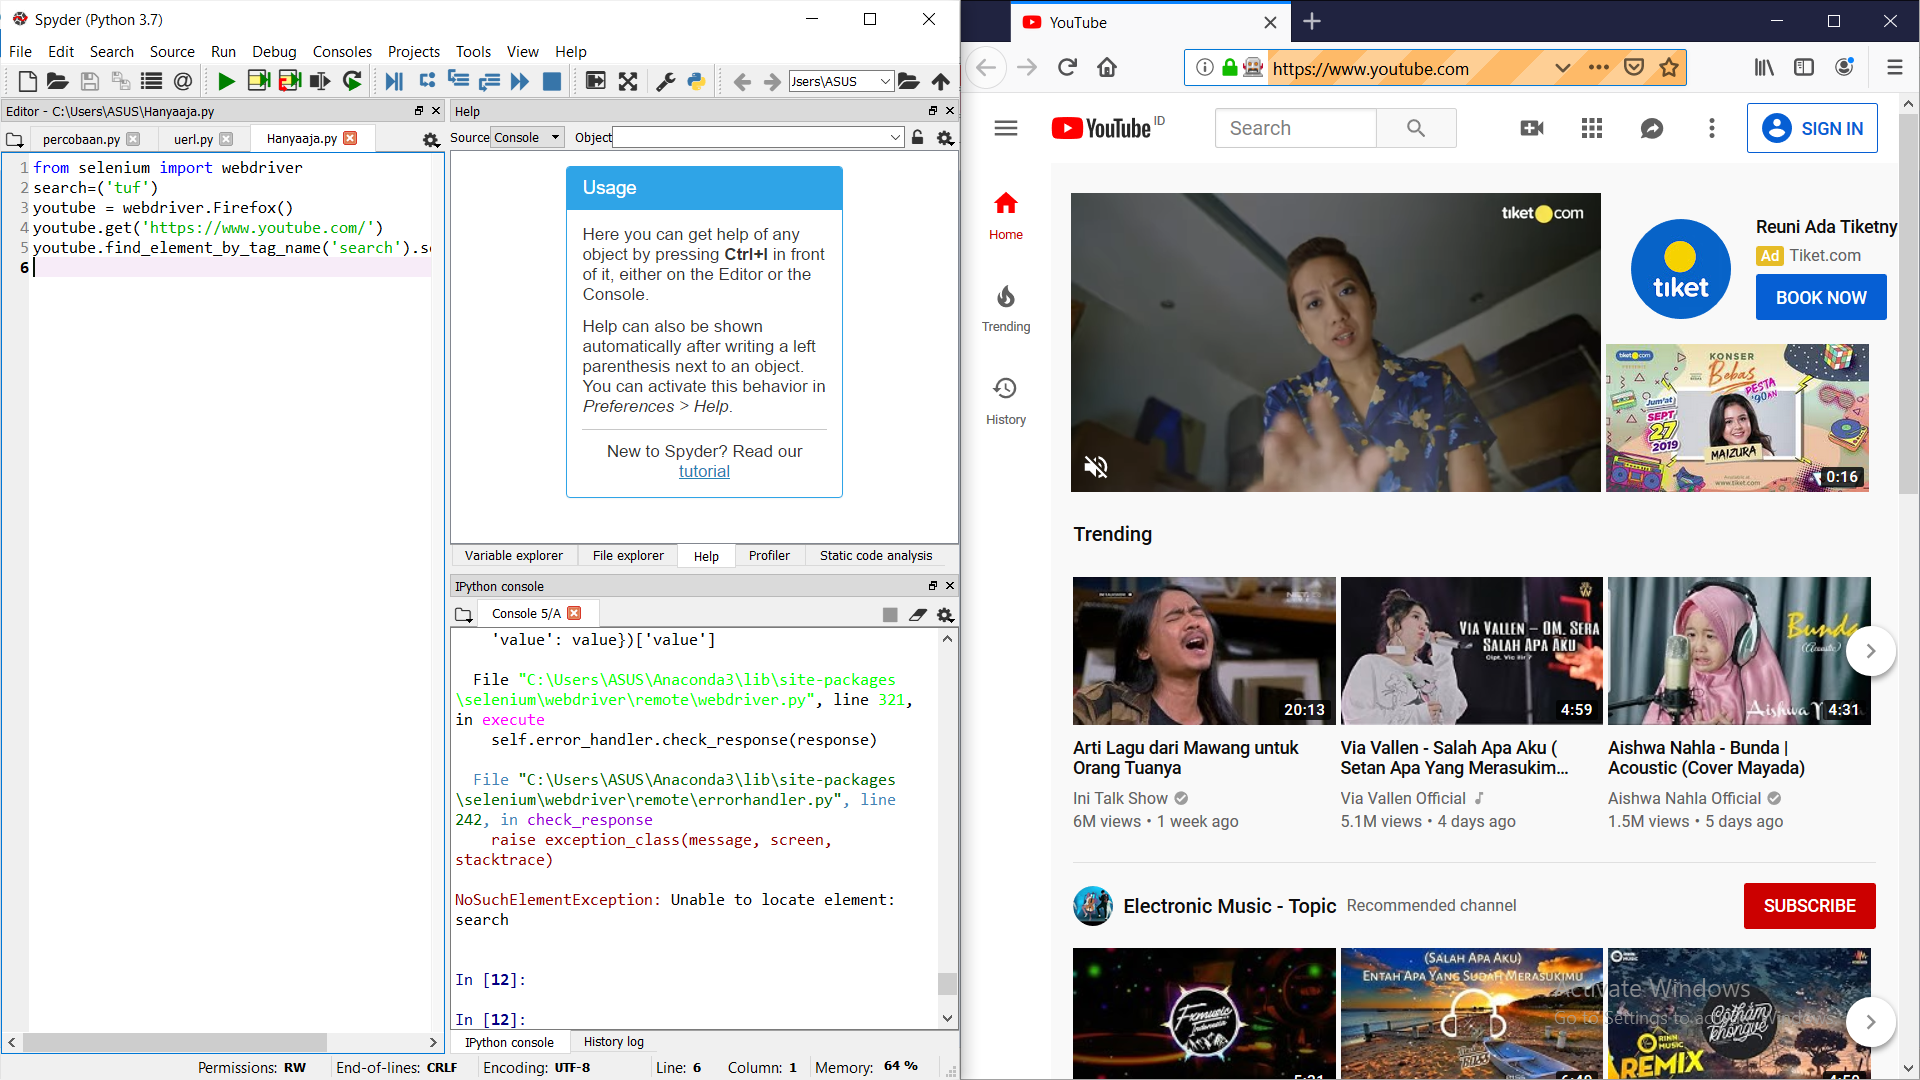
\includegraphics[scale=0.3]{figure/hasilTes/7.png}
    \label{gambar 1}
\end{figure}

\vspace{6cm}
    
    \item Kita menggunakan find\_element\_by\_xpath sebagai Pemberikan text secara otomatis. Saat  Di run hasil pada menu search pada youtube tidak muncul text yang telah ditentukan. Dan pada Spyder {(unable to locate search element)}
\begin{figure}[!htbp]
    \centering
    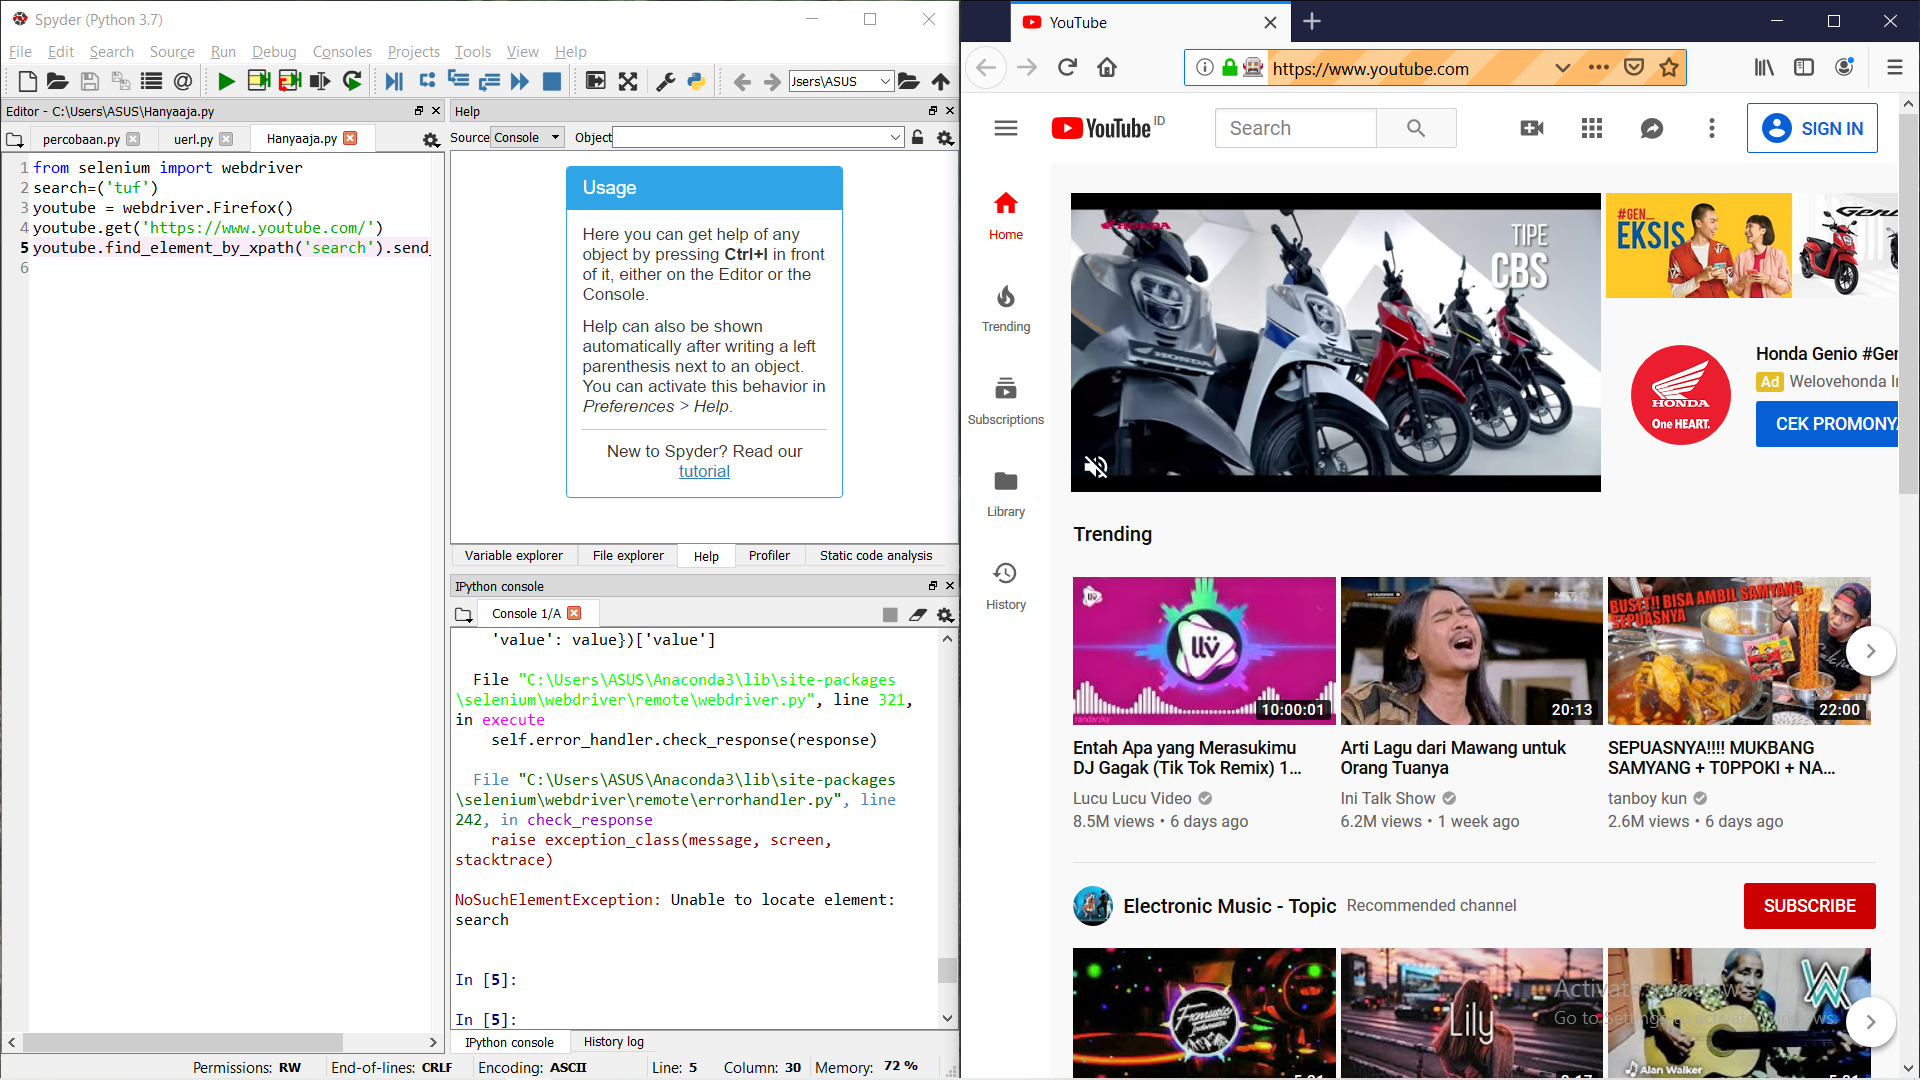
\includegraphics[scale=0.3]{figure/hasilTes/8.png}
    \label{gambar 1}
\end{figure}

    \item Kita menggunakan find\_elements sebagai Pemberikan text secara otomatis. Saat  Di run hasil pada menu search pada youtube tidak muncul text yang telah ditentukan. Dan pada Spyder {(unknown variant 'search')}
\begin{figure}[!htbp]
    \centering
    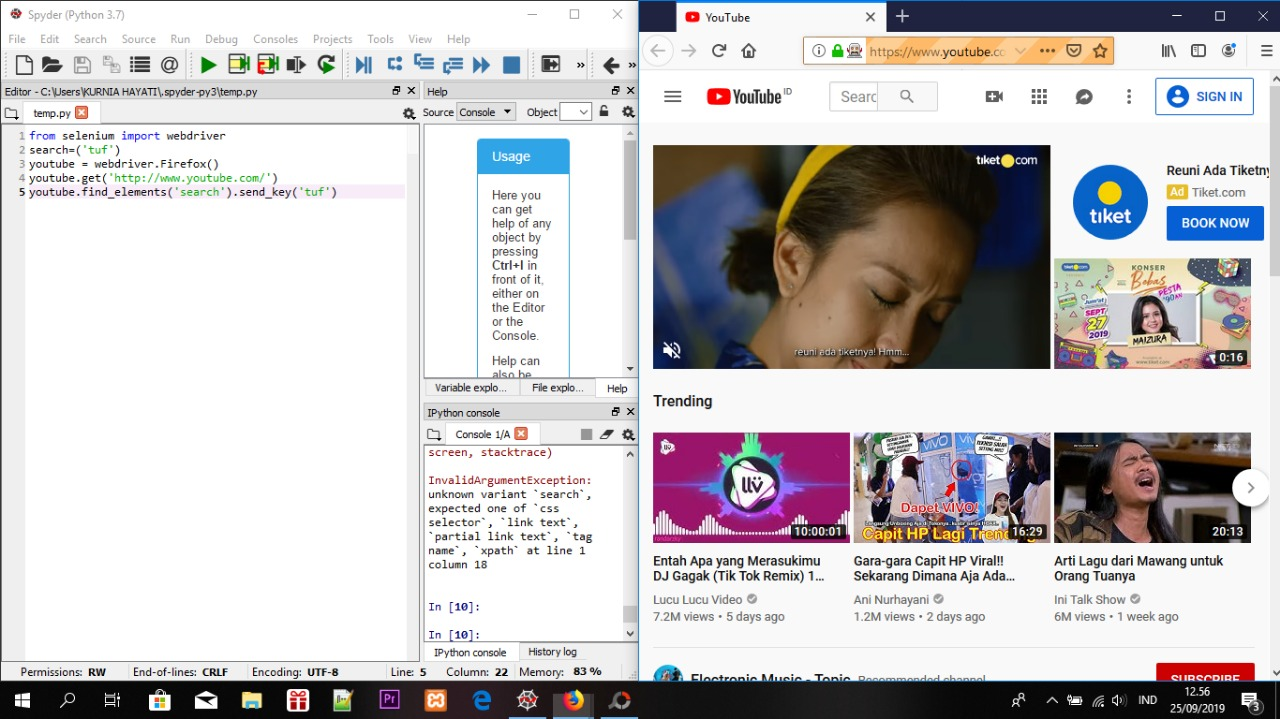
\includegraphics[scale=0.3]{figure/hasilTes/9.jpg}
    \label{gambar 1}
\end{figure}

    \item Kita menggunakan find\_elements\_by\_css\_selector sebagai Pemberikan text secara otomatis. Saat  Di run hasil pada menu search pada youtube tidak muncul text yang telah ditentukan. Dan pada Spyder {(list object has not attribut send\_key)}
\begin{figure}[!htbp]
    \centering
    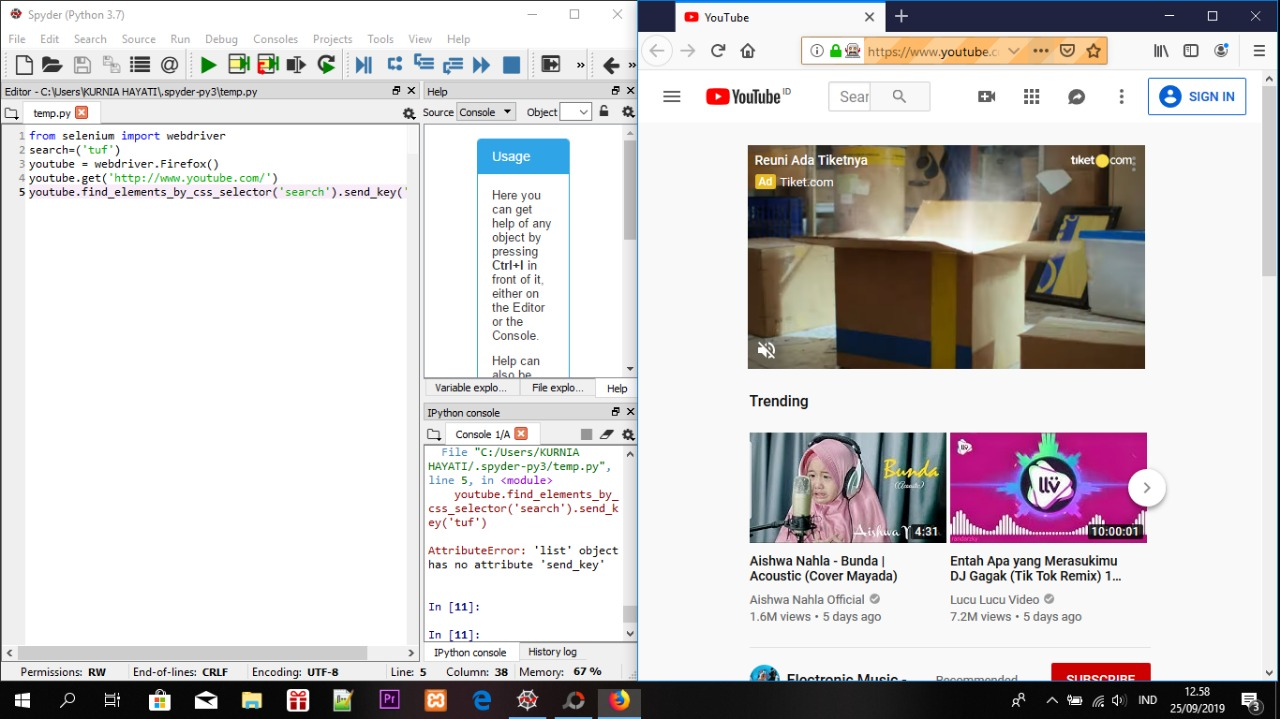
\includegraphics[scale=0.3]{figure/hasilTes/10.jpeg}
    \label{gambar 1}
\end{figure}

    \item Kita menggunakan find\_elements\_by\_name sebagai Pemberikan text secara otomatis. Saat  Di run hasil pada menu search pada youtube tidak muncul text yang telah ditentukan. Dan pada Spyder {(unable to locate search element)}
\begin{figure}[!htbp]
    \centering
    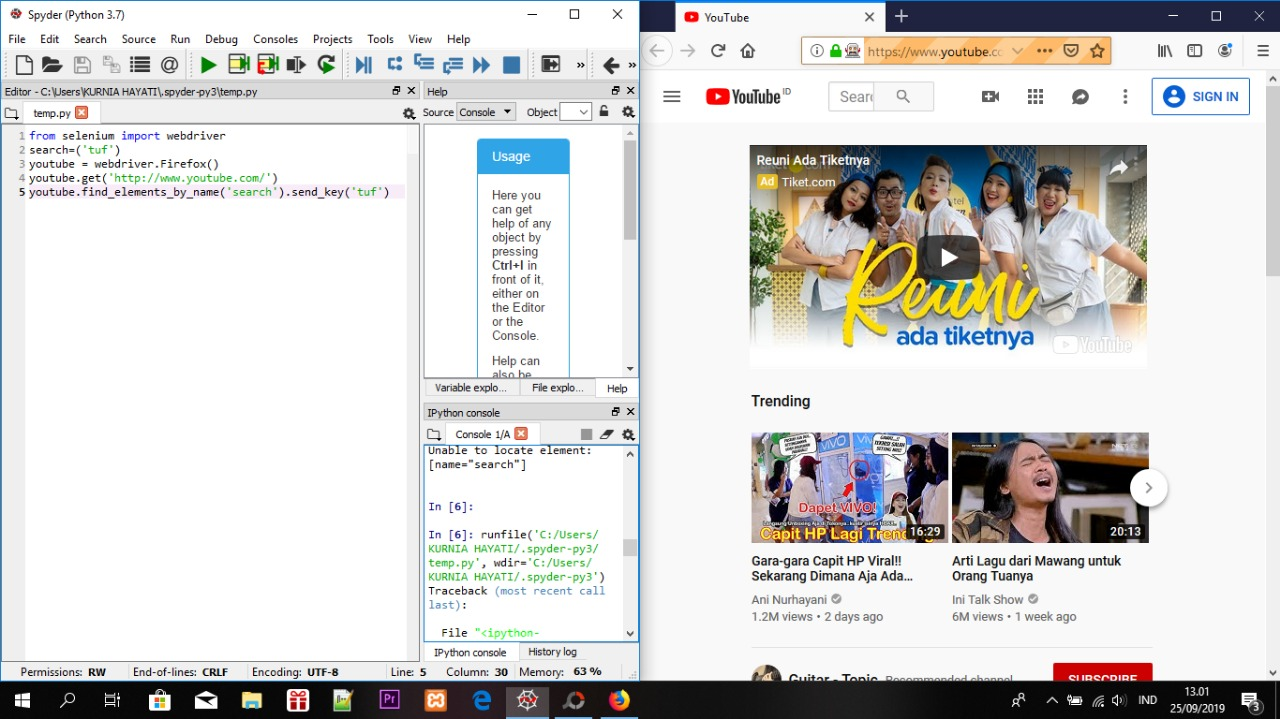
\includegraphics[scale=0.3]{figure/hasilTes/11.jpeg}
    \label{gambar 1}
\end{figure}

    \item Kita menggunakan find\_elements\_by\_partial\_link\_text sebagai Pemberikan text secara otomatis. Saat  Di run hasil pada menu search pada youtube tidak muncul text yang telah ditentukan. Dan pada Spyder {(unable to locate search element)}
\begin{figure}[!htbp]
    \centering
    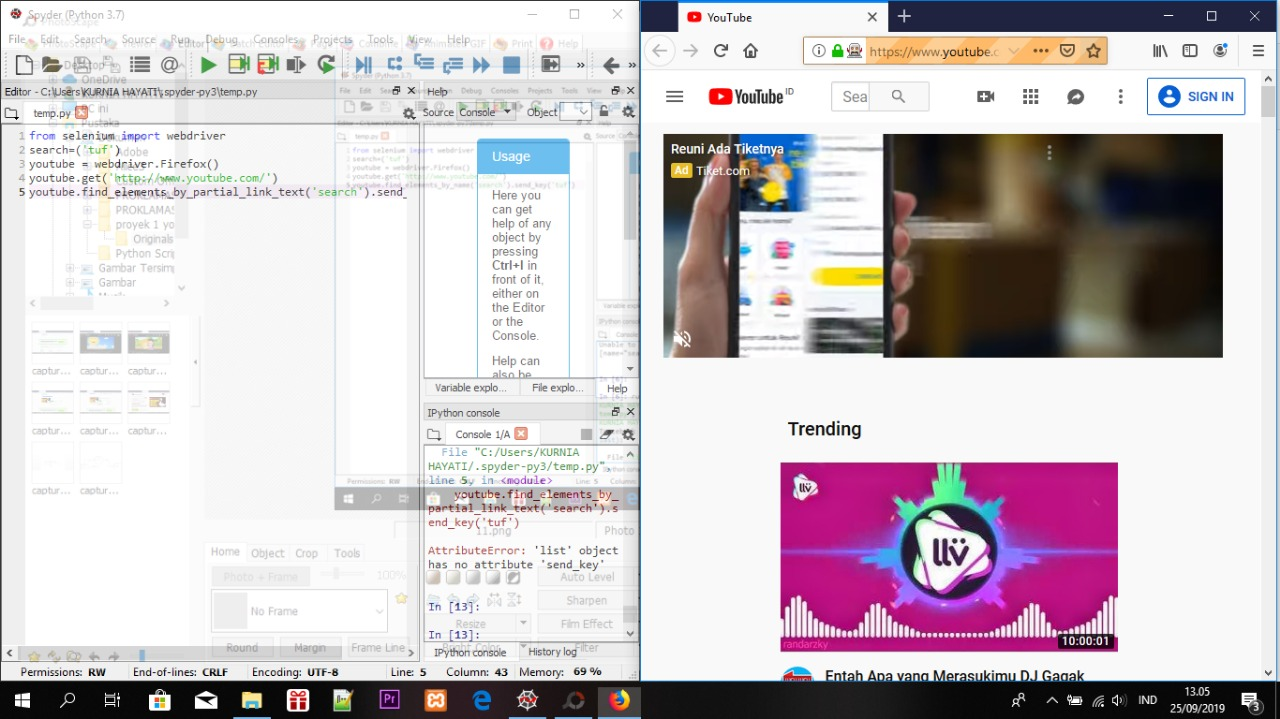
\includegraphics[scale=0.3]{figure/hasilTes/12.jpeg}
    \label{gambar 1}
\end{figure}

\vspace{1cm}

    \item Kita menggunakan find\_elements\_by\_tag\_name sebagai Pemberikan text secara otomatis. Saat  Di run hasil pada menu search pada youtube tidak muncul text yang telah ditentukan. Dan pada Spyder {(list object has not attribut send\_key)}
\begin{figure}[!htbp]
    \centering
    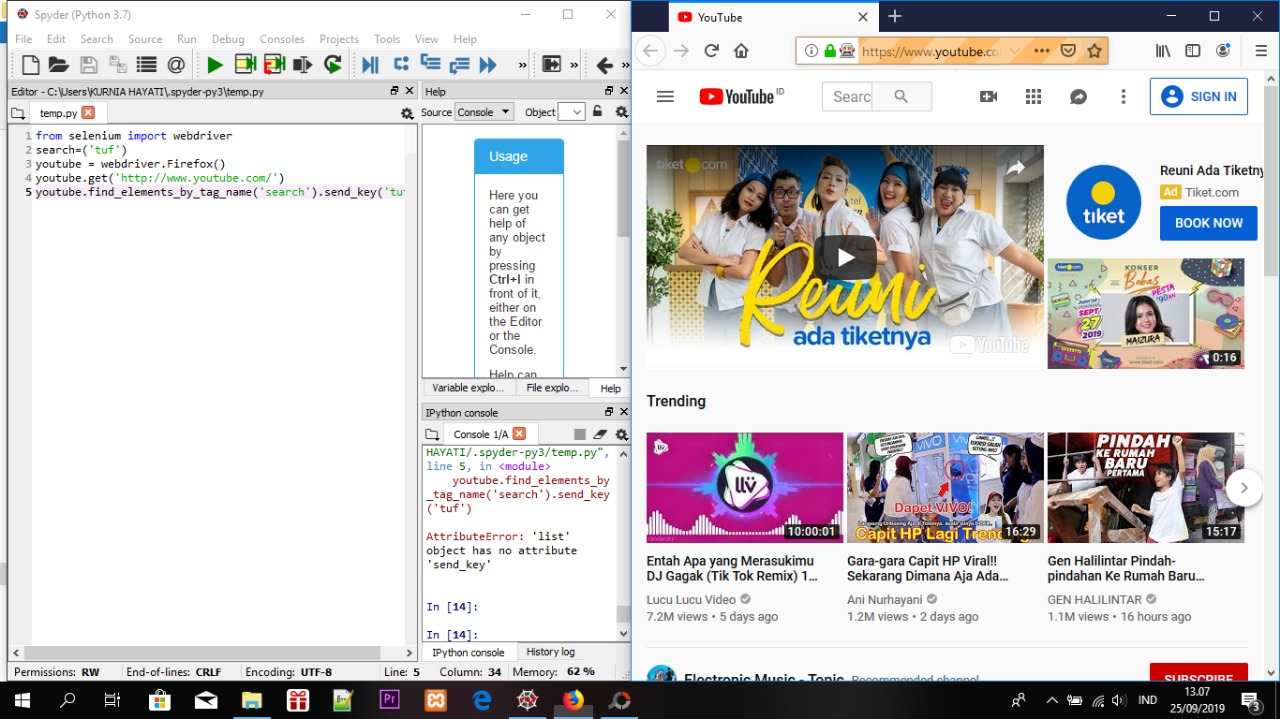
\includegraphics[scale=0.3]{figure/hasilTes/13.jpeg}
    \label{gambar 1}
\end{figure}

    \item Kita menggunakan find\_elements\_by xpath sebagai Pemberikan text secara otomatis. Saat  Di run hasil pada menu search pada youtube tidak muncul text yang telah ditentukan. Dan pada Spyder {(list object has not attribut send\_key)}
\begin{figure}[!htbp]
    \centering
    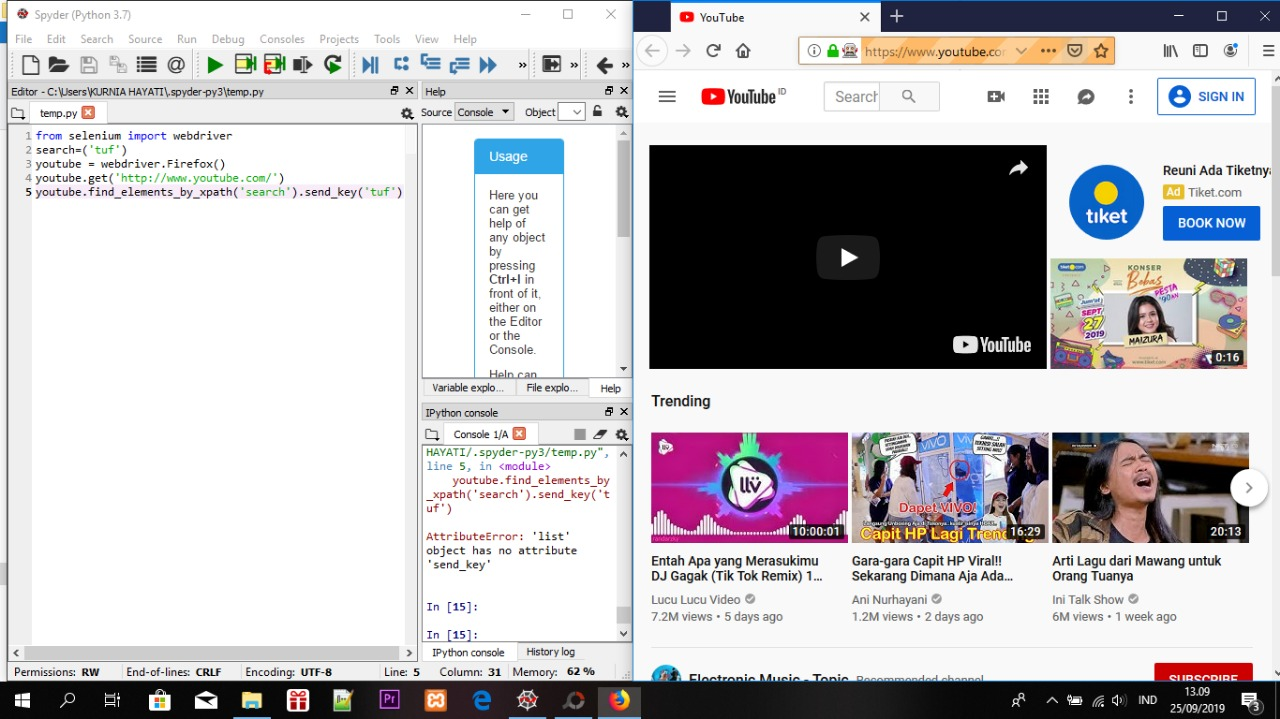
\includegraphics[scale=0.3]{figure/hasilTes/14.jpeg}
    \label{gambar 1}
\end{figure}
\end{enumerate}

\subsection{Hasil Pengujian}
Hasil dari uji diatas dengan berberapa cara tidak berhasil dalam memberikan text pada menu pencarian pada youtube sehingga pada code program selenium spyder (Anaconda 3) diubah dapat diliahat sebagi berikut:

\begin{figure}[!htbp]
    \centering
    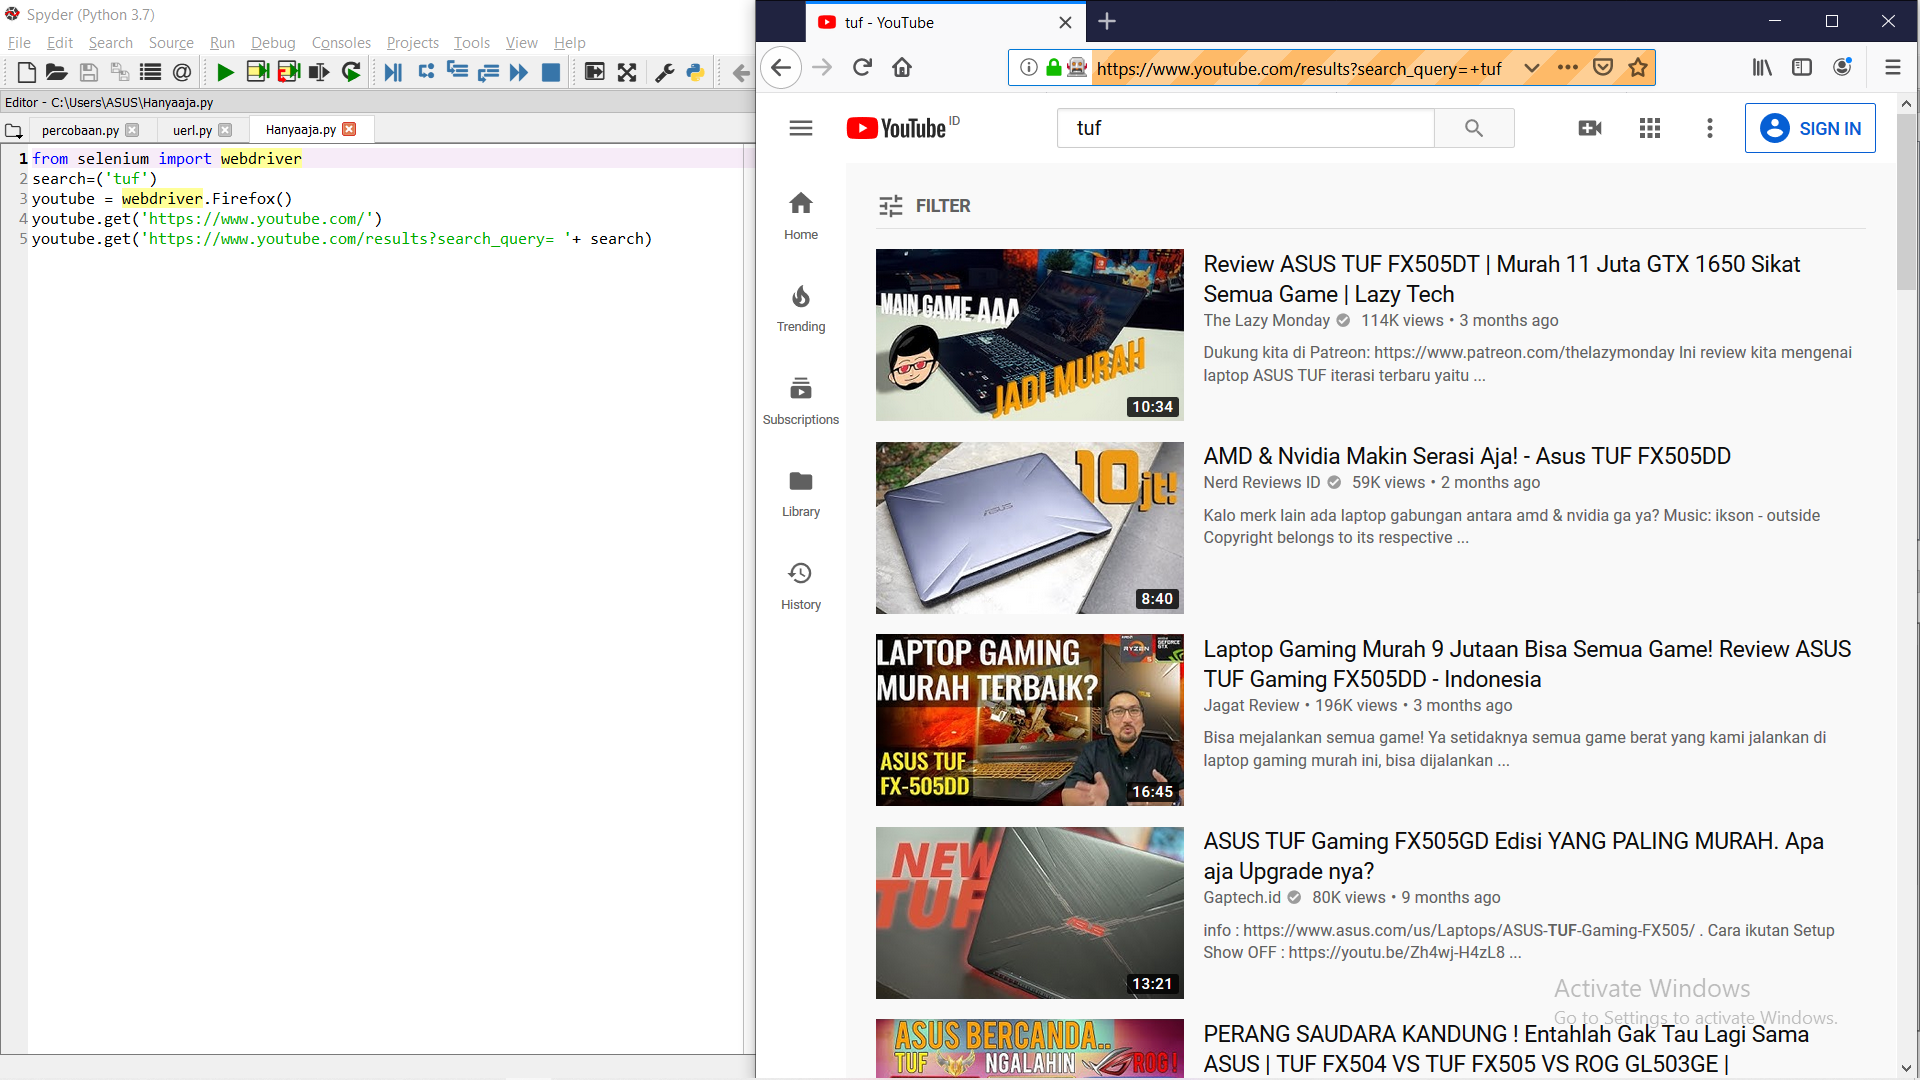
\includegraphics[scale=0.3]{figure/akhirnya.png}
    \label{gambar 1}
\end{figure}

\begin{enumerate}
    \item Dimana ditambahkan variable search dimana berfungsi sebagi media pencarian judul video yang akan dicari.
    \item Kemudia pada youtube.get('https://www.youtube.com/results?search\_query= '+ search)
    Ditambahkan dengan simbol + dengan variable search telah dibuat.
\end{enumerate}
 
\chapter{Kesimpulan dan Saran}

\section{Kesimpulan}
Kesimpulan yang dapat diambil dari hasil Analisis Aplikasi Downloader Mp4 ini adalah sebagai berikut:
\begin{enumerate}
    \item Berdasarkan analisis yang ada  kita mengetahui bagaimana sistem yang berjalan dari awal pencarian video youtube hingga mendownload video dengan aplikasi MP4 Youtube (savefrom.net).
    \item Melalui analisis ini kita juga bisa mengetahui bagaimana menjalankan sebuah program secara otomatis dengan bantuan selenium.
\end{enumerate}
\section{Saran}
Saran yang disampaikan oleh penulis yang daoat digunakan sebagai bahan pertimbangan bagi aplikasi downloader MP4 youtube dan Youtube sendiri masih ada bagian yang sulit untuk di  ketahui dimana pada menu \textit {search} {(pencarian)}pada youtube tidak menemukan element yang sesuai sehingga tidak bisa menggunakan element yang tersedia pada aplikasi pendukung selenium spyder {(Anaconda 3)}. sehingga dapat lebih memaksimalkan lagi dalam memenuhi kebutuhan pengguna . Serta agar dapat dilakukan pengembangan dan perbaikan secara berkesinambungan pada analisis berikutnya. 
\include{section/chapter6} 

%now enable appendix numbering format and include any appendices
%\appendix
%\include{section/appendix1}
%\include{section/appendix2}

%next line adds the Bibliography to the contents page
\addcontentsline{toc}{chapter}{Daftar Pustaka}
%uncomment next line to change bibliography name to references
%\renewcommand{\bibname}{References}
\bibliography{references}        %use a bibtex bibliography file refs.bib
\bibliographystyle{plain}  %use the plain bibliography style

\end{document}

